\documentclass{article}

% Conditional compilation.
% NOTE: If you set fullversionfalse, just compile ONCE so that TOC stays unchanged.
\newif\iffullversion
\fullversiontrue
%\fullversionfalse


%%%%%%%%%%%%%%%%%%%%%%%%%%%%%%%%%%%%%%%%%%%%%%%%%%%%%%%%%%%%%%%%%%%%%%%%%
\pagestyle{plain}                                                      %%
%%%%%%%%%% EXACT 1in MARGINS %%%%%%%                                   %%
\setlength{\textwidth}{6.5in}     %%                                   %%
\setlength{\oddsidemargin}{0in}   %% (It is recommended that you       %%
\setlength{\evensidemargin}{0in}  %%  not change these parameters,     %%
\setlength{\textheight}{8.5in}    %%  at the risk of having your       %%
\setlength{\topmargin}{0in}       %%  proposal dismissed on the basis  %%
\setlength{\headheight}{0in}      %%  of incorrect formatting!!!)      %%
\setlength{\headsep}{0in}         %%                                   %%
\setlength{\footskip}{.5in}       %%                                   %%
%%%%%%%%%%%%%%%%%%%%%%%%%%%%%%%%%%%%                                   %%
\newcommand{\required}[1]{\section*{\hfil #1\hfil}}                    %%
\renewcommand{\refname}{\hfil References Cited\hfil}                   %%
\bibliographystyle{plain}                                              %%
%%%%%%%%%%%%%%%%%%%%%%%%%%%%%%%%%%%%%%%%%%%%%%%%%%%%%%%%%%%%%%%%%%%%%%%%%

\usepackage{graphicx}
\usepackage{color}

\pagestyle{empty}

\begin{document}

\large

\vbox{}
\begin{figure}[!ht]
%\hspace{-4mm}

\includegraphics[width=8cm]{img/logo.png}
\vspace{18mm}
\end{figure}

\begin{figure}[!ht]
\begin{center}
%\hspace{-4mm}
%\hspace{-20mm}
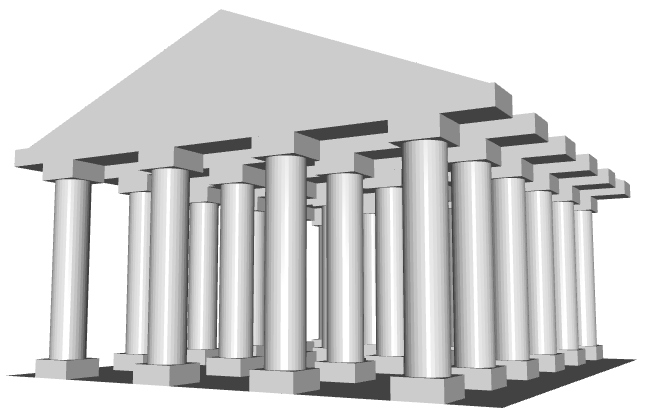
\includegraphics[width=8cm]{img/plasm-temple.png}\hspace{1cm}
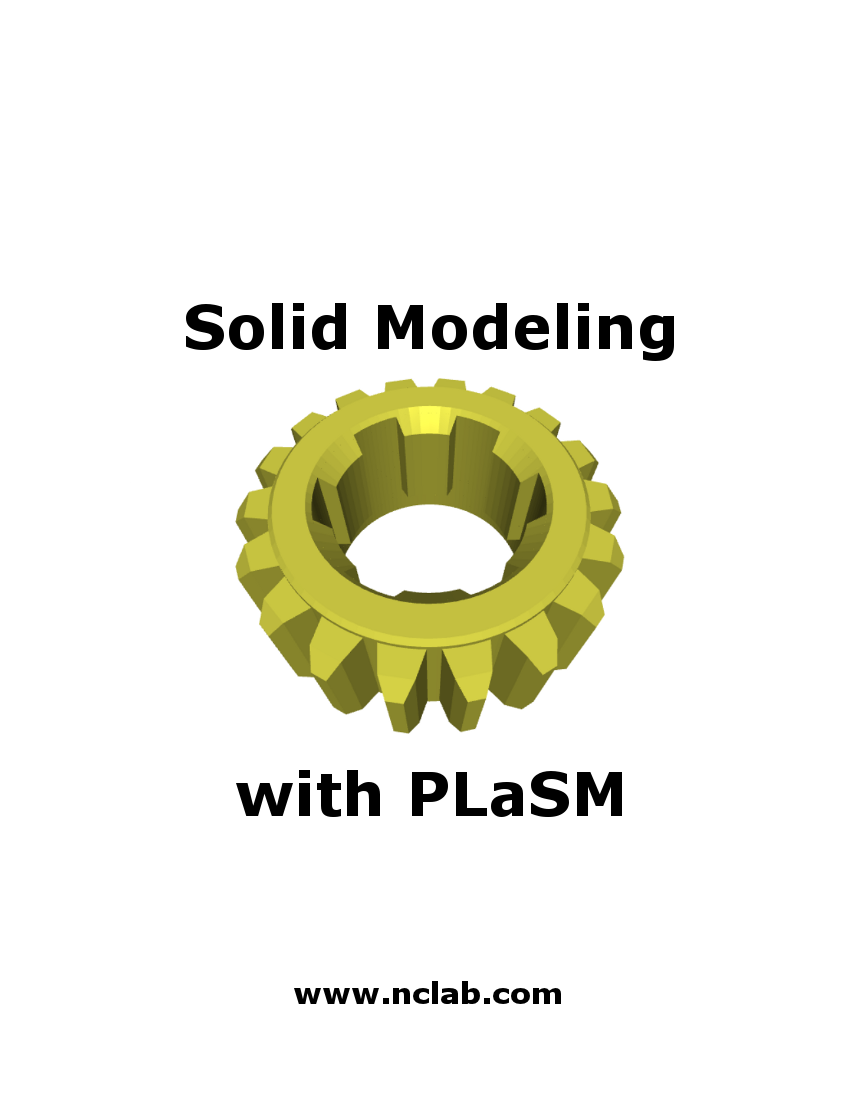
\includegraphics[width=5.5cm]{img/plasm-frontpage.png}
\vspace{12mm}
\end{center}
\end{figure}

\begin{center}
{\Huge \bf Solid Modeling with PLaSM}\\
\vbox{}
\vspace{1cm}
\iffullversion
\else
\centerline{\huge \color{red}{PREVIEW}}
\fi
\vfill
{\large
{\bf Pavel Solin \& Salih Dede}
}
\end{center}
\vfill
\vfill
\begin{center}
Copyright 2012 FEMhub Inc. All rights reserved.
\end{center}
\newpage

%%%%%%%%%%%%%%%%%%%%%%%%%%%%%%%%%%%%%%%%%%%%%%%%%%%%%%%%%%%%%%%%%%%%%%%%%

\vbox{}
\vfill
{
\noindent
{\bf About this Textbook}\\[4mm]
This textbook is provided as a courtesy to you and all other NCLab users. 
It will help you discover the elegance and power of Solid Modeling which 
forms the basis of modern CAD systems.  \\[12mm]

\noindent
{\bf About the Authors}\\[4mm]
Pavel Solin is Professor of Computational Mathematics at the University of Nevada, Reno. 
As part of his profession, he has been developing advanced computer programs in various 
programming languages for
many years, and also supervising the development of large open-source projects related to 
high-performance scientific computing. Salih Dede is Instructor of Computer
Programming at the Coral Academy of Science High School in Reno. He has vast experience 
with teaching programming to high school students, and outstanding instructional
achievements. \\[12mm]


\noindent
{\bf For Instructors}\\[4mm]
Review Book and Exercise Book containing 
hundreds of review questions with answers and programming exercises with
solutions, respectively, are part of the NCLab-powered course 
{\em Intro to Programming with Karel the Robot and Python} that is 
available at \\

\centerline{\tt http://introtoprogramming.net}
\vspace{5mm}

\noindent
for a small subscription fee.  In addition to 
standard cloud benefits such as anytime-anywhere accessibility through 
the web browser interface and working from mobile devices, the course comes with 
additional attractive features including 
automated grading and student progress tracking. 
The course will be opened in August 2012.
}
\vfill





%%%%%%%%%%%%%%%%%%%%%%%%%%%%%%%%%%%%%%%%%%%%%%%%%%%%%%%%%%%%%%%%%%%%%%%%%
\newpage

\pagestyle{plain}
\setcounter{page}{1}

\section{Getting Started}

\subsection{Objectives}
\begin{itemize}
\item Learn basic facts about Solid Modeling and PLaSM.
\item Understand how to clone and display projects.
\item As a "Hello, World!" example, wreate a unit cube.
\item Learn to rotate, move and zoom objects displayed via WebGL.
\end{itemize}

\subsection{Solid Modeling and PLaSM}

Solid Modeling (SM) is a consistent set of principles for mathematical and computer 
modeling of three-dimensional solids. Solid Modeling is distinguished from related 
areas such as geometric modeling or computer graphics by its emphasis on {\em physical fidelity}.
SM is the basis of computer-aided design (CAD), engineering simulations, and other disciplines.

PLaSM ({\em Programming Language for Solid Modeling}) is a simple and elegant design 
language backed up with powerful computational geometry algorithms. It 
enables geometrical modeling of 3D objects via simple commands.
The language was developed by the CAD Group at the Universities of Roma 
"La Sapienza" and "Roma Tre" in Italy. It is based on FL, an advanced 
language for functional programming developed at the IBM Research Center.

PLaSM makes it possible to define a wide range of simple 3D objects, transform 
them, create intersections and unions via simple logical operations, and much 
more. This textbook will guide you in small steps and using many examples
through Solid Modeling with the help of PLaSM. Soon, you will be able to create 
advanced 3D geometries such as the one shown in Fig. \ref{fig:pisa}.

\begin{figure}[!ht]
\begin{center}

\includegraphics[width=0.7\textwidth]{img/temple0.png}
\end{center}
\vspace{-4mm}
\caption{Sample PLaSM model (available as Displayed Project "Temple").}
\vspace{-1cm}
\label{fig:pisa}
\end{figure}
\newpage
\subsection{How does NCLab work}

NCLab is the underlying cloud computing platform for this course. Operation with the 
PLaSM library is done through a simple {\em scripting language}, meaning that  
objects are created, transformed, and manipulated via {\em simple commands} rather 
than by clicking into menus of some graphical application. The scripts are 
sent to a remote cloud server, evaluated there, and the results are sent back
to your web browser. Some tasks such as Boolean operations with 3D objects 
(their intersections, unions etc.) may require heavy computing and take some time.
This, however, is not done on your computer or laptop. Your device only uses 
its graphics card for real-time rendering of 3D objects. For this reason, {\bf your 
web browser has to support WebGL}.

\subsection{Displayed projects}

All examples that we are going to work with in the following are also available 
as Displayed Projects. This means that you can clone them by launching the File
Manager, going to the {\em Project} menu, and clicking on {\em Clone}. This will 
launch a window with many displayed projects. Look for projects whose names start 
with "PLaSM - Tutorial". After you locate a project that you would like to clone, 
click on it, and then click on the button {\em Clone} at the bottom of the window. 
This will create an exact copy of that project in your account. You can open it,
edit, run, save, and do whatever you like with it. Your changes will not affect 
the original Displayed Project. Vice versa, you are welcome to display your own 
projects if you think that other users might find them interesting!


\subsection{Launching a new PLaSM project}

Alternatively to cloning examples into your account, you can type them. This is 
recommended since you become more fluent in using the scripting language. 
Most of the introductory examples are very short anyway. New PLaSM projects 
can be launched via the CAD icon on Desktop, as shown in Fig. \ref{fig:python}.
\newpage

\begin{figure}[!ht]
\begin{center}
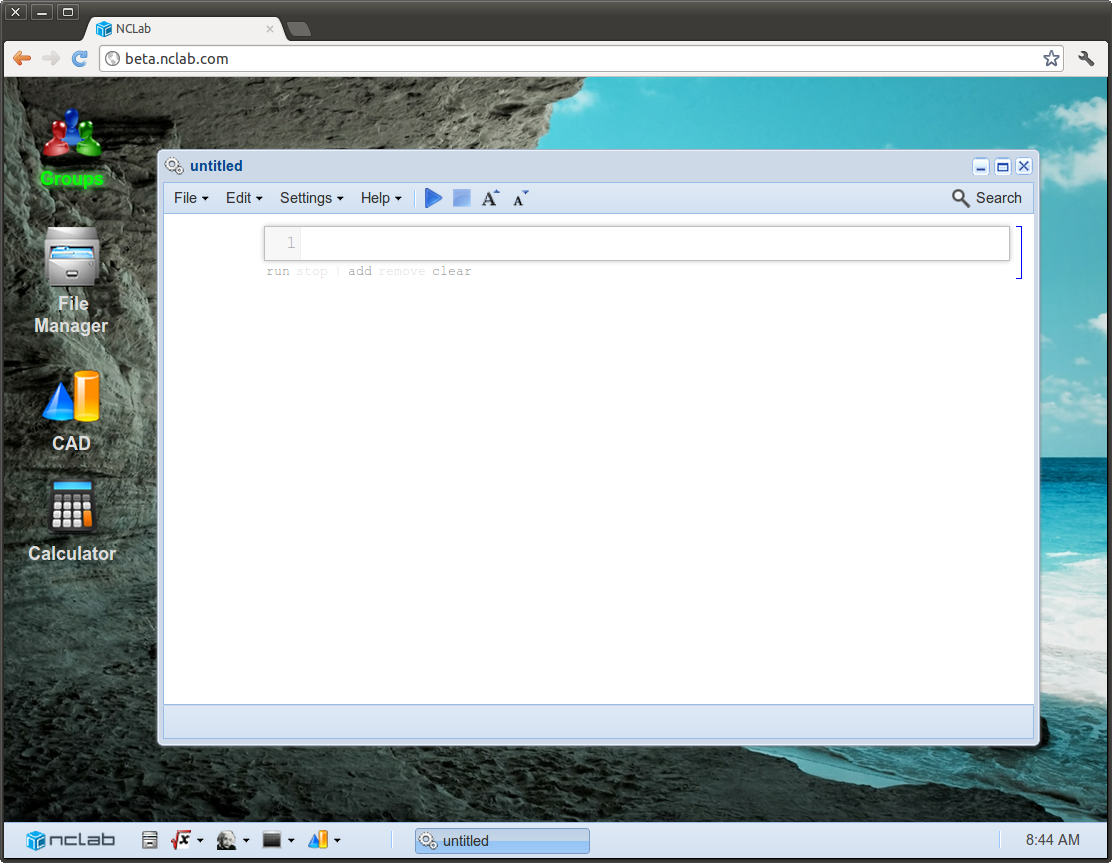
\includegraphics[width=\textwidth]{img/python.png}
\end{center}
%\vspace{-2mm}
\caption{Launching a new PLaSM project.}
\label{fig:python}
\end{figure}
\noindent

\subsection{Hello, World!}

In the input cell, enter the code:

\begin{verbatim}
from pyplasm import *
cube = CUBE(1)
lab.view(cube, [0.4, 0.9, 0.6])
\end{verbatim}
Here, {\tt CUBE} is a command that creates a cube, its parameter is the edge length,
and {\tt cube} is the name of the object.
The name can be arbitrary as long as it does not conflict with any PLaSM command. 
To minimize name clashes, all PLaSM commands are CAPITALIZED.
The three numbers enclosed in square brackets define a color in the 
OpenGL format. The numbers stand for red (R), green (G) and blue (B) 
components of the resulting color, and each value is between 0 (darkest) and 
1 (lightest). For example, [0, 0, 0] means black, [1, 1, 1] means white. 
More about colors will be said in Subsection \ref{subsec:colors}.

After you are done typing the script, click on the 'run' button in the menu 
or under the input cell. The former option will run all cells 
in the project, the latter only the one selected cell. This will send the script to a remote
server. The answer should come back instantly, and a new WebGL widget displaying a unit cube 
will appear, as shown in Fig. \ref{fig:cube}. 

\begin{figure}[!ht]
\begin{center}
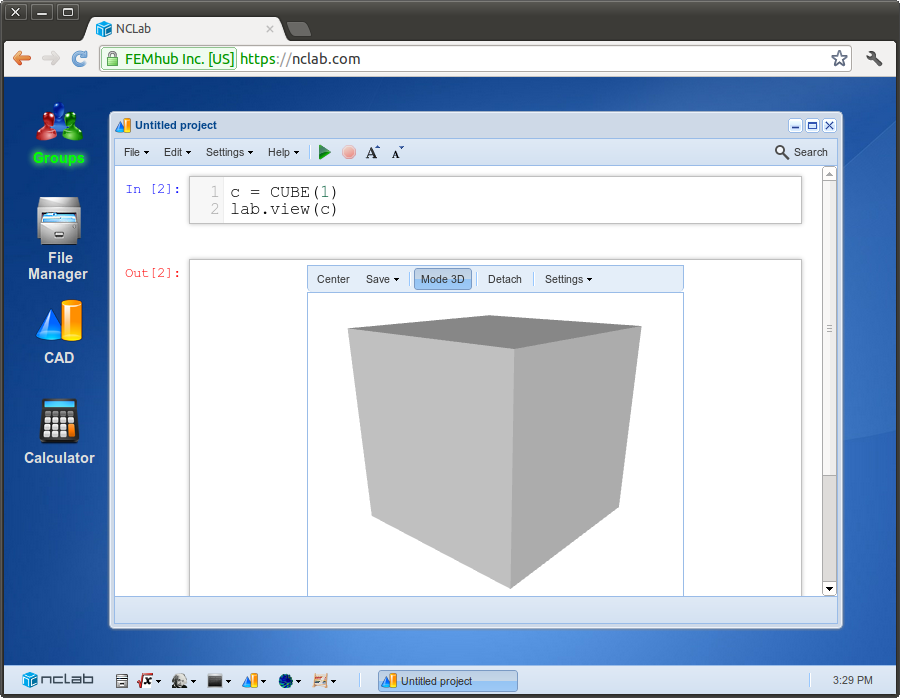
\includegraphics[width=\textwidth]{img/cube.png}
\end{center}
\vspace{-2mm}
\caption{WebGL widget showing the unit cube that we created.}
\vspace{2mm}
\label{fig:cube}
\end{figure}
\noindent
Congratulations, you just 
created your first Solid Model!\\

\noindent
Before we move on, let us briefly explain the above code.
The first line, 

\begin{verbatim}
from pyplasm import *
\end{verbatim}
imports the PLaSM library. The prefix "py" stands for Python (NCLab uses
Python to call PLaSM). The second line,

\begin{verbatim}
cube = CUBE(1)
\end{verbatim}
defines a unit cube. Cube of a general edge length {\tt e} would be 
created by replacing the number {\tt 1} with {\tt e}. The last line,

\begin{verbatim}
lab.view(cube, [0.4, 0.9, 0.6])
\end{verbatim}
displays the cube in a WebGL widget, using a greenish color. 

\subsection{Mouse controls}

Now click into the window and move the mouse while holding the left
button down. The cube will rotate freely. Holding the middle
button (or the mouse wheel) pressed and moving the mouse will move the 
object in any direction. Zooming in and out is done via the mouse wheel 
or by holding the right-hand mouse button down and moving the mouse.
The latter option allows for finer zooming.

\subsection{Review questions}

\begin{enumerate}
\item How does Solid Modeling differ from Computer Graphics?
\begin{itemize}
\item[A1] There is no difference, they are the same thing. 
\item[A2] Computer graphics represents 3D onjects more precisely.
\item[A3] Solid Modeling represents 3D objects more precisely.
\item[A4] Solid Modeling is used primarily for 3D animations.
\end{itemize}
\item What does the abbreviation CAD stand for?
\begin{itemize}
\item[A1] Computer-assisted drawing.
\item[A2] Computer-allowed discrepancy.
\item[A3] Computer-aided design.
\item[A4] Computer-amplified drumming.
\end{itemize}
\item What is PLaSM?
\begin{itemize}
\item[A1] Make of plasma 3D TVs.
\item[A2] Computer graphics library.
\item[A3] Design language backed up with powerful computational geometry algorithms.
\item[A4] Browser plugin for rendering 3D objects.
\end{itemize}
\item In NCLab, scripts are evaluated:
\begin{itemize}
\item[A1] On the user's computer.
\item[A2] In the user's web browser.
\item[A3] On a remote server.
\item[A4] Using the user's graphic card.
\end{itemize}
\item What can you do with a Displayed Project that you clone?
\begin{itemize}
\item[A1] View but not run or edit or save.
\item[A2] View and run but not edit or save.
\item[A3] View, edit and run but not save.
\item[A4] View, edit, run, save. 
\end{itemize}
\item How can a PLaSM script be evaluated?
\begin{itemize}
\item[A1] By hitting ENTER.
\item[A2] By clicking on "run" under the input cell.
\item[A3] By clicking on the blue arrow button.
\item[A4] By clicking on Run in the File menu.
\end{itemize}
\item How is PLaSM imported into the project?
\begin{itemize}
\item[A1] {\tt from plasm import *}
\item[A2] {\tt from pyplasm import *}
\item[A3] {\tt from plasm import pyplasm}
\item[A4] {\tt from pyplasm import plasm}
\end{itemize}
\item What of the following is the correct way to create a cube of edge length $e$?
\begin{itemize}
\item[A1] {\tt c = C(e)}
\item[A2] {\tt c = CB(e)}
\item[A3] {\tt c = CUBE(e)}
\item[A4] {\tt c = HEXAHEDRON(e)}
\end{itemize}
\item What color is represented by the triplet [1, 1, 1]?
\begin{itemize}
\item[A1] Black
\item[A2] White
\item[A3] Green
\item[A4] Magenta.
\end{itemize}
\item How can we visualize an object {\tt c} using the color [0.9, 0.9, 0.9]?
\begin{itemize}
\item[A1] {\tt lab.visualize(c, [0.9, 0.9, 0.9])}
\item[A2] {\tt lab.show(c, [0.9, 0.9, 0.9])}
\item[A3] {\tt lab.view(c, [0.9, 0.9, 0.9])}
\item[A4] {\tt lab.display(c, [0.9, 0.9, 0.9])}
\end{itemize}
\end{enumerate}

\subsection{Exercises}

\begin{enumerate}
\item Write a PLaSM script to render a unit cube in pure red color.
\item Write a PLaSM script to render a cube of edge length 2 in pure green color.
\item Write a PLaSM script to render a cube of edge length 3 in pure blue color.
\end{enumerate}

\newpage
\section{Creating Simple Objects}

\subsection{Objectives}
\begin{itemize}
\item Understand RGB colors.
\item Create squares, rectangles, cubes and bricks.
\item Learn to always remember where objects are positioned in the coordinate system.
\item Create convex hulls.
\item Understand the benefits of scripting.
\item Create triangles, tetrahedra and prisms.
\item Create a cone via convex hull.
\item Create cylinders and tubes.
\item Create spheres and toruses.
\end{itemize}


\subsection{Using RGB colors} \label{subsec:colors}

The triplet {\tt [0.4, 0.9, 0.6]} that was used in the {\tt lab.view()} command
above represented the RGB components of a greenish color. The color can be changed 
by redefining these three numbers. The numbers can be arbitrary as long as they stay 
between 0.0 and 1.0. You can experiment with various colors, keeping a few 
simple rules in mind:

\begin{itemize}
\item With just the first value being non-zero, such as in {\tt [0.5, 0, 0]},
      you get {\bf red} color. The closer the value is to 1.0, the lighter the color
      will be.
\item With just the second value being non-zero, such as in {\tt [0, 0.5, 0]},
      you obtain {\bf green} color. The closer the  value is to 1.0, the lighter the color
      will be.
\item With just the third value being non-zero, such as in {\tt [0, 0, 0.5]},
      you will have {\bf blue} color. The closer the  value is to 1.0, the lighter the color
      will be.
\item Using three identical values will result into some shade of grey. For 
      example, {\tt [0.0, 0.0, 0.0]}
      means black and {\tt [1.0, 1.0, 1.0]} means white.
\item Varying all three numbers, you can get any color that you want. It is not 
      easy to translate a color, such as "purple", "cyan" or "orange" into the RGB
      values. But there are many web pages that will do it for you, such as for
      example http://kb.iu.edu/data/aetf.html. {\bf Note}: Usually,
      the RGB values on these web pages are given as integers between 0 and 255. To use them in NCLab,
      just divide all three of them by 255.
\end{itemize}

 
\subsection{Brick, cube, rectangle, and square -- commands CUBE, CUBOID}

We already know the command {\tt CUBE} that takes one positive real
parameter (the edge length) and renders a 3D cube. We can use a more general command {\tt CUBOID}
to render bricks, cubes, rectangles and squares.
   
With three parameters {\tt a, b, c} enclosed in square brackets, the {\tt CUBOID} command will 
render a 3D brick with edge lengths {\tt a}, {\tt b} and {\tt c}. To illustrate this, 
change the code in your input cell to  

\begin{verbatim}
from pyplasm import *
cube = CUBOID([3, 2, 1])
lab.view(cube, [0.4, 0.9, 0.6])
\end{verbatim}
and run the input cell. The result is displayed in Fig. \ref{fig:cuboid-1}.


\begin{figure}[!ht]
\begin{center}
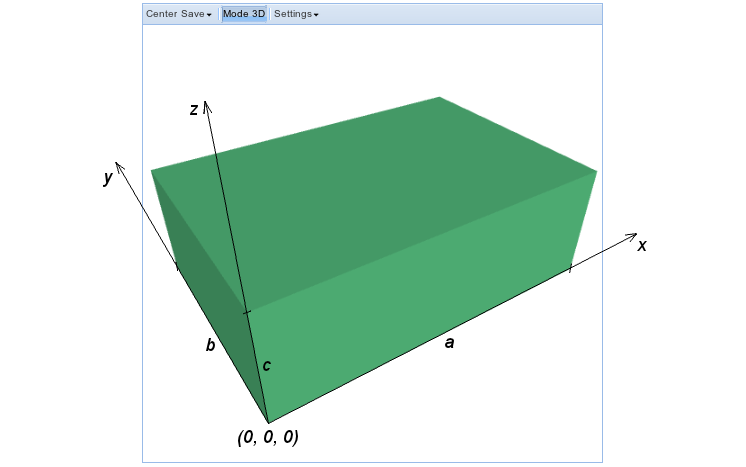
\includegraphics[width=0.8\textwidth]{img/cuboid-1.png}
\end{center}
\vspace{-2mm}
\caption{CUBOID([3, 2, 1]) generates a brick with edge lenghts 3, 2 and 1.}
\label{fig:cuboid-1}
\end{figure}
\noindent
Fig. \ref{fig:cuboid-1} also shows coordinate axes which are not
displayed in the WebGL widget. As you can see, the brick is positioned 
in the first quadrant, its edges are aligned with coordinate axes, and one 
vertex lies at the origin (0, 0, 0). In order to avoid mistakes when working with 
multiple objects, it is very important to always remember where
each object is located in the global coordinate system. 

With two parameters {\tt [a, b]} the CUBOID command will render a 2D rectangle 
with edge lengths {\tt a} and {\tt b}, as shown in Fig. \ref{fig:cuboid-2}.

\newpage

\begin{figure}[!ht]
\begin{center}
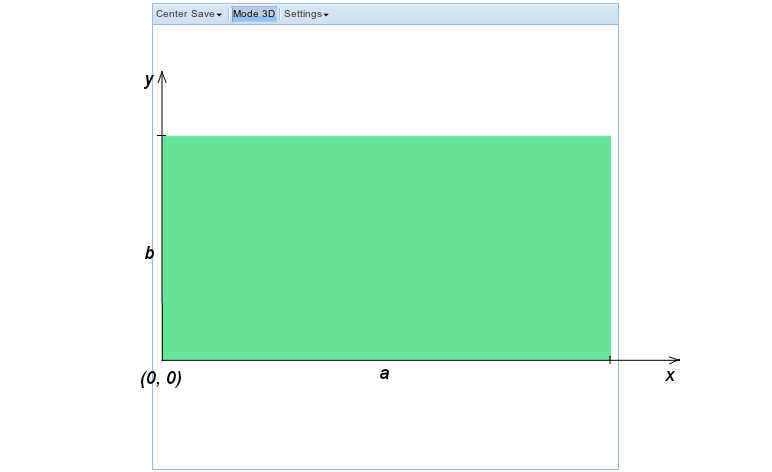
\includegraphics[width=0.82\textwidth]{img/cuboid-2.png}
\end{center}
\vspace{-2mm}
\caption{CUBOID([2, 1]) generates a rectangle with edge lenghts 2 and 1.}
\label{fig:cuboid-2}
%\vspace{-1cm}
\end{figure}
\noindent
Notice again that the rectangle is located in the first quadrant with its edges 
aligned with coordinate axes, and that its bottom-left vertex lies at the 
origin (0, 0).

\subsection{Unit tetrahedron and triangle -- command SIMPLEX}

Unit tetrahedron (unit 3D simplex) can be created using the 
{\tt SIMPLEX(3)} command:
\begin{verbatim}
from pyplasm import *
tet = SIMPLEX(3)
lab.view(tet, [0.4, 0.9, 0.6])
\end{verbatim}
The simplex spans the points (0, 0, 0), (1, 0, 0), (0, 1, 0) and (0, 0, 1),
as depicted in Fig. \ref{fig:simplex-1}.
\newpage

\begin{figure}[!ht]
\begin{center}
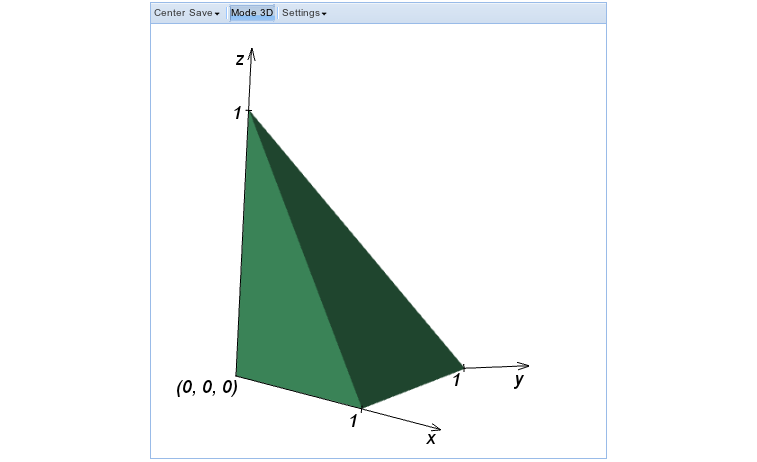
\includegraphics[width=0.82\textwidth]{img/simplex-1.png}
\end{center}
\vspace{-2mm}
\caption{SIMPLEX(3) generates a unit 3D simplex (unit tetrahedron).}
\label{fig:simplex-1}
\end{figure}
\noindent
Unit triangle (unit 2D simplex) can be created using the code
\begin{verbatim}
from pyplasm import *
tria = SIMPLEX(2)
lab.view(tria, [0.4, 0.9, 0.6])
\end{verbatim}
The simplex spans the points (0, 0), (1, 0) and (0, 1), as shown in 
Fig. \ref{fig:simplex-2}.
\newpage

\begin{figure}[!ht]
\begin{center}
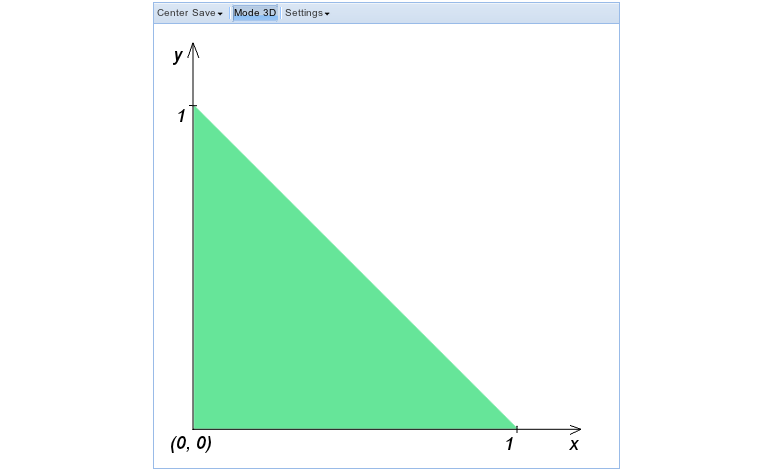
\includegraphics[width=0.82\textwidth]{img/simplex-2.png}
\end{center}
\vspace{-2mm}
\caption{SIMPLEX(2) generates a unit 2D simplex (unit triangle).}
\label{fig:simplex-2}
%\vspace{-1cm}
\end{figure}
\noindent

\subsection{Command CONVEXHULL}\label{par:chull}

The command CONVEXHULL is a powerful tool to define convex 2D and 3D objects
that span a given list of 2D and 3D points, respectively. The command takes 
a single parameter which is a list of points. For example, the code

\begin{verbatim}
from pyplasm import *
points = [[-1, 0], [1, 0], [0.5, 1], [-0.5, 1]]
t = CONVEXHULL(points)
lab.view(t, [0.4, 0.9, 0.6])
\end{verbatim}
will render a 2D trapezoid spanning the points (-1, 0), (1, 0), (0.5, 1) and 
(-0.5, 1). The code

\begin{verbatim}
from pyplasm import *
points = [[-1, -1, 0], [1, -1, 0], [1, 1, 0], [-1, 1, 0], [0, 0, 1]]
p = CONVEXHULL(points)
lab.view(p, [0.4, 0.9, 0.6])
\end{verbatim}
creates a 3D pyramid with base square (-1, 1)$\times$(-1, 1) and height 1,
as shown in Fig. \ref{fig:pyra}.
\newpage

\begin{figure}[!ht]
\begin{center}
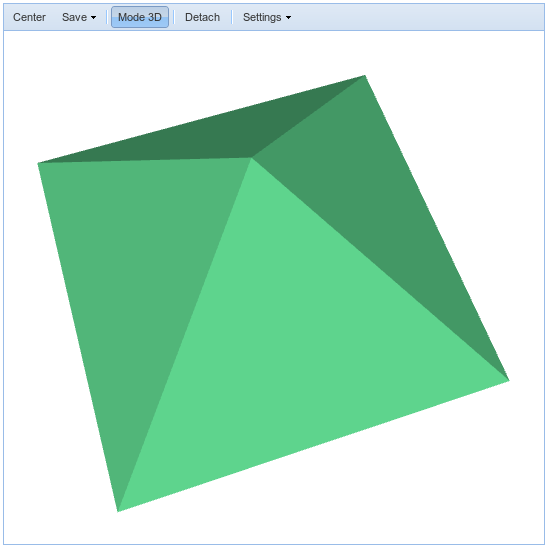
\includegraphics[width=0.5\textwidth]{img/pyra.png}
\end{center}
\vspace{-2mm}
\caption{3D pyramid constructed as a convex hull.}
\label{fig:pyra}
%\vspace{-1cm}
\end{figure}
\noindent


\subsection{General tetrahedron and triangle via convex hull}

The command CONVEXHULL can be used to create general triangles and 
tetrahedra. For example, the code

\begin{verbatim}
from pyplasm import *
points = [[1, 1], [4, 2], [2, 4]]
tria = CONVEXHULL(points)
lab.view(tria, [0.4, 0.9, 0.6])
\end{verbatim}
generates a triangle with vertices (1, 1), (4, 2) and (2, 4). The code

\begin{verbatim}
from pyplasm import *
points = [[-2, 0, 0], [1, 0, 0], [0, 4, 1], [0, 1, 2]]
tet = CONVEXHULL(points)
lab.view(tet, [0.4, 0.9, 0.6])
\end{verbatim}
creates a tetrahedron with vertices (-2, 0, 0), (1, 0, 0), (0, 4, 1) and (0, 1, 2),
as shown in Fig. \ref{fig:chull}.
\newpage

\begin{figure}[!ht]
\begin{center}
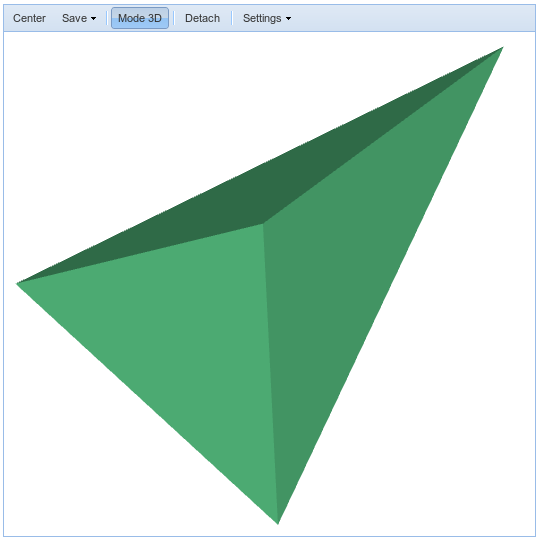
\includegraphics[width=0.5\textwidth]{img/chull.png}
\end{center}
\vspace{-2mm}
\caption{General tetrahedron obtained via convex hull.}
\label{fig:chull}
%\vspace{-1cm}
\end{figure}
\noindent

\subsection{The power of scripting unleashed}

By {\em scripting} we mean designing solid objects via 
short programs. The main benefit of scripting is that we can 
create {\em parameter-dependent geometries}. This is 
very useful in practice since in most cases some parameters of 
the design at hand need tuning. Such as, for example, the 
number of teeth on a gear, thickness of a wall, size of an
opening, distance between two objects, etc.

PLaSM is very strong in scripting. Let us learn a bit 
more about Python so that we are able to take maximum advantage 
of what PLaSM can offer. We already know a few Python commands, 
for example:

\begin{verbatim}
from pyplasm import *
\end{verbatim} 
which imports all functionality from the PLaSM library.\\

\noindent
\underline{Defining variables}\\

\noindent
Whenever we need to tune a parameter in our design, we can create 
a variable for it. Imagine that we have to create a brick whose base
is (0, 3)$\times$(0, 2) but whose exact height will be determined 
later. Hence  we create a new variable {\tt h} for the height and initialize 
it with some reasonable value, such as for example with {\tt 1.0}:

\begin{verbatim}
h = 1.0
\end{verbatim} 
The rest we already know:

\begin{verbatim}
from pyplasm import *
b = CUBOID([3, 2, h])
lab.view(a, [0.4, 0.9, 0.6])
\end{verbatim} 
This will render a brick of dimensions 3$\times$2$\times$1. Now it is easy to 
change the height of the brick without changing the script that defines it --
the script will remain the same, only the value of the variable {\tt h} needs
to be changed:

\begin{verbatim}
a = 5.0
\end{verbatim} 
After the script is run again, we have a new brick of dimensions 3$\times$2$\times$5.\\

\noindent
\underline{Numpy library}\\

\noindent
We are free to use Python libraries for our designs, remarkably Numpy. 
Numpy contains vast functionality related to 
mathematical functions and numerical computations. Whenever we want 
to use some constant such as $\pi$ or $e$, or when we want to use some 
mathematical function such as log$(x)$, sin$(x)$ or $\sqrt{x}$, we
import it from Numpy:

\begin{verbatim}
from numpy import log, sin, sqrt
\end{verbatim} 
We can also simply import everything:

\begin{verbatim}
from numpy import *
\end{verbatim} 
\vspace{4mm}
\underline{Python lists}\\

\noindent
Whenever we need to create a set of objects, such as a set of points, we can use 
a Python list for that. Empty Python list is created using square brackets that 
contain nothing in them:

\begin{verbatim}
L = []
\end{verbatim} 
Here, {\tt L} is the name of the list, and any other name would be fine as well, 
as long as it does not clash with some Python or PLaSM command. We can also create 
a nonempty list. Say that we need a list that contains the points (0, 0), (1, 0),
(1, 0). This is done via:

\begin{verbatim}
L = [[0, 0], [1, 0], [0, 1]]
\end{verbatim} 
Yes you are right, each point is a list in fact! Sometimes we need to fill 
a list using some procedure because not all its items are known at the
beginning. For this, we can use the command {\tt append()}. For example,
one more point (2, 4) is added to the existing list {\tt L} via

\begin{verbatim}
L.append([2, 4])
\end{verbatim} 
\vspace{4mm}
\underline{Printing}\\

\noindent
Control prints are a practical way to check that all numbers are as they should be.
Printing is done via the {\tt print} command. For example, the script

\begin{verbatim}
L = [[0, 0], [1, 0], [0, 1]]
print L
\end{verbatim} 
has the following output:

\begin{verbatim}
[[0, 0], [1, 0], [0, 1]]
\end{verbatim} 
Printing the value of a single variable is done in the same way, and we can 
make the output more informative by actually describing what is printed.
The script

\begin{verbatim}
h = 5.0
print "h =", h
\end{verbatim} 
yields the following output:

\begin{verbatim}
h = 5.0
\end{verbatim} 
\vspace{4mm}
\underline{Repeating}\\

\noindent
Let us mention one last scripting technique for now, which is to repeat 
some command or sequence of commands several times. To repeat something 
{\tt N} times, we use the following construct: 

\begin{verbatim}
for i in range(0, N):
    do_something
\end{verbatim}
For example, the following script will print a sequence of integers between 
0 and 5 (not including 5):

\begin{verbatim}
for i in range(0, 5):
    print i
\end{verbatim}
Output:

\begin{verbatim}
0
1
2
3
4
\end{verbatim}
Once more -- notice that the printed sequence ends with {\tt 4}, not with {\tt 5}.
This is a common source of beginner's mistakes.
Also notice that the command(s) to be repeated need to be indented. The indent is mandatory and 
its size can be either two or four empty characters -- four is recommended for better
code readability.

Let us show one more example of how repetition can be used: We will create a list of 
points (0, 0), (1, 0), (2, 0), ..., (N, 0) where {\tt N} is some positive integer. Let us
write the script initially for {\tt N = 5}, and at the end we will print it:

\begin{verbatim}
N = 5
L = []
for i in range(0, N+1):
    L.append([i, 0])
print "L =", L
\end{verbatim}
Output:
\begin{verbatim}
L = [[0, 0], [1, 0], [2, 0], [3, 0], [4, 0], [5, 0]]
\end{verbatim}
If we needed to create another list for {\tt N = 100}, the script would remain the same,
just the line where {\tt N} is defined would be changed to 

\begin{verbatim}
N = 100
\end{verbatim}
We can see clearly that scripting can save us lots of work.

\subsection{Polygon via convex hull}\label{subsec:polygon}

Next we will write a simple script that generates 
a polygon with $N$ equally-long edges that is inscribed in 
a circle of radius $R$. With the knowledge of Python 
gained in the previous paragraph, you should understand 
the following script easily. The only new thing worth 
mentioning is that points 

\begin{verbatim}
[R * cos(angle), R * sin(angle)]
\end{verbatim}
where {\tt angle} is an angle between $0$ and $2\pi$, lies
on the circle with center (0, 0) and radius $R$:

\begin{verbatim}
from pyplasm import *
from numpy import sin, cos, pi
N = 15
R = 5
points = []
for i in range(N):
    angle = i * 2. * pi / N
    points.append([R * cos(angle), R * sin(angle)])
polygon = CONVEXHULL(points)
lab.view(polygon, [0.4, 0.9, 0.6])
\end{verbatim}
The output of the above code is shown in Fig. \ref{fig:convexhull-1}.

\newpage

\begin{figure}[!ht]
\begin{center}
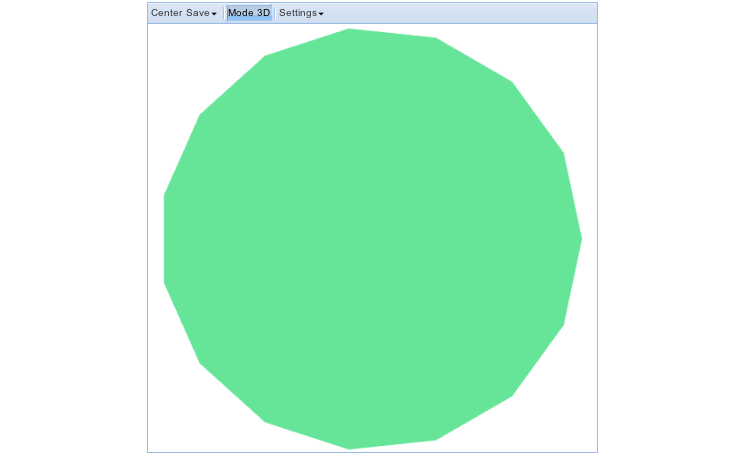
\includegraphics[width=0.82\textwidth]{img/convexhull-1.png}
\end{center}
\vspace{-2mm}
\caption{Polygon with 15 equally long edges inscribed into a circle.}
\label{fig:convexhull-1}
%\vspace{-1cm}
\end{figure}

\subsection{Circle via convex hull}\label{par:cico}

When the parameter $N$ is increased to 128 or 256 in the program from 
Subsection \ref{subsec:polygon}, one obtains a {\bf circle}. This 
circle is enough for now. Later, in Section \ref{sec:cso2}, we will 
introduce a more rigorous definition of a circle based on {\em reference 
maps}. 

\subsection{Cone via convex hull}\label{par:coco}

The CONVEXHULL command has amazing power. Let us tweak the script
from Subsection \ref{subsec:polygon} to construct a cone of radius
$R$ and height $H$. All we need to do is to add a zero third coordinate 
to the points generated in that script, and add one more point -- the 
tip of the cone. The CONVEXHULL command will take care of the rest:

\begin{verbatim}
from pyplasm import *
from numpy import sin, cos, pi
R = 5
H = 10
points = []
subdiv = 128
for i in range(N):
    angle = i * 2. * pi / subdiv
    points.append([R * cos(angle), R * sin(angle), 0])
points.append([0, 0, H])
cone = CONVEXHULL(points)
lab.view(cone, [0.4, 0.9, 0.6])
\end{verbatim}
\noindent
The output is shown in Fig. \ref{fig:convexhull-2}.

\begin{figure}[!ht]
\begin{center}
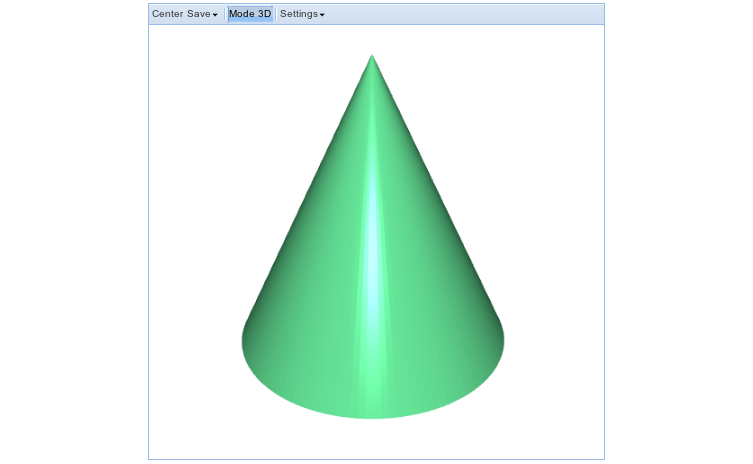
\includegraphics[width=0.82\textwidth]{img/convexhull-2.png}
\end{center}
\vspace{-2mm}
\caption{Cone of radius $R$ and height $H$.}
\label{fig:convexhull-2}
%\vspace{-1cm}
\end{figure}
\noindent
\underline{How fine subdivision?}\\

\noindent
The subdivision {\tt subdiv = 128} is how many
faces are used to approximate the round surface. You may use less, 
for example 64 or even 32, which will make the rendering faster, but
the surface will be less smooth. With more than 
128 subdivisions the surface will be even more smooth-looking, but 
the rendering will take longer. We do not recommend going over 128 
subdivisions as it is not necessary.

\subsection{Command PRISM}

Given any 2D polygon {\tt B} and a positive number {\tt H}, the command {\tt PRISM(H)(B)} 
creates a prism with basis {\tt B} and height {\tt H}. For example, the 
following code creates a prism of height $2.0$ whose basis is a triangle 
with vertices (-1, 0), (1, 0), (0, 2):

\begin{verbatim}
from pyplasm import *
B = CONVEXHULL([[-1, 0], [1, 0], [0, -2]])
H = 2.0
p = PRISM(H)(B)
lab.view(p, [0.4, 0.9, 0.6])
\end{verbatim}
The output is shown in Fig. \ref{fig:prism}.

\begin{figure}[!ht]
\begin{center}
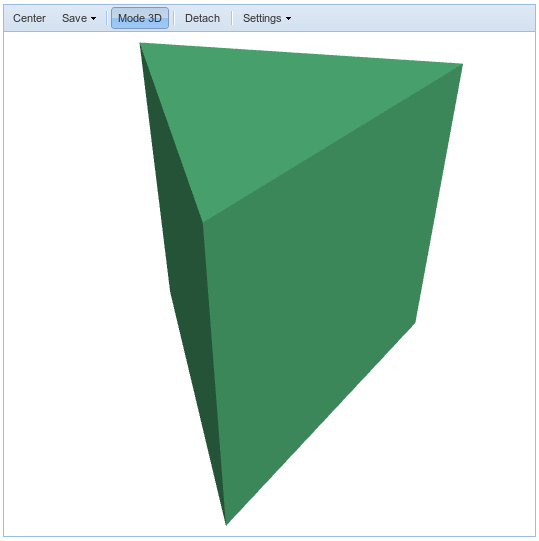
\includegraphics[width=0.5\textwidth]{img/prism-0.png}
\end{center}
\vspace{-2mm}
\caption{Triangular prism of height $H$.}
\label{fig:prism}
%\vspace{-1cm}
\end{figure}

\subsection{Command CYLINDER}

A cylinder of radius $R$ and height $H$ is a convex object 
and thus it would be easy to construct it via convex hull. 
But, PLaSM has a specific command CYLINDER for that:

\begin{verbatim}
from pyplasm import *
R = 0.25
H = 1.0
subdiv = 128
cyl = CYLINDER ([R, H])(subdiv)
lab.view(cyl, [0.4, 0.9, 0.6])
\end{verbatim}
Notice that the radius {\tt R} and height {\tt H} are entered  
as a single Python list {\tt [R, H]}, and that a subdivision parameter 
{\tt subdiv} is present. We already know its meaning -- this is the 
number of linear segments to approximate the curved vertical part
of the cylinder's surface. 

The positioning of the object in the global 
coordinate system is important -- the cylinder's axis is in 
the $z$-direction, and the midpoint of its base circle is the 
origin (0, 0, 0). The output is shown in Fig. \ref{fig:cyl-1}.
\newpage

\begin{figure}[!ht]
\begin{center}
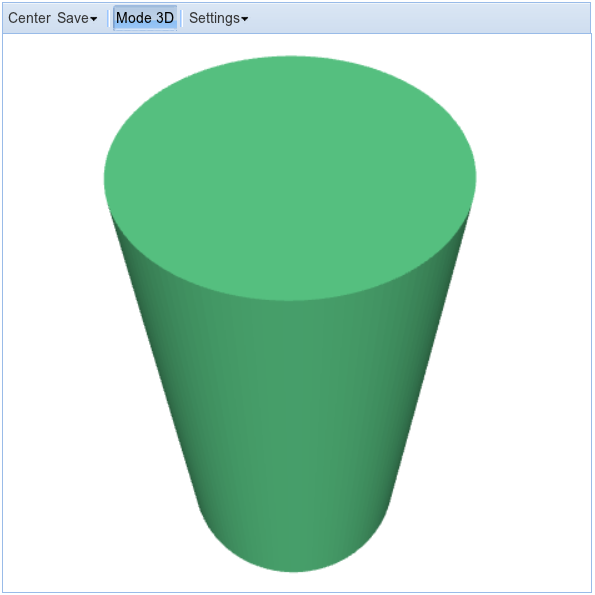
\includegraphics[width=0.5\textwidth]{img/cyl-1.png}
\end{center}
\vspace{-2mm}
\caption{Cylinder of radius $R$ and height $H$.}
\label{fig:cyl-1}
%\vspace{-1cm}
\end{figure}

\subsection{Command TUBE}

A hollow tube of inner radius $r$, outer radius $R$ and height
$H$ is rendered using the TUBE command. It is used as follows:
\begin{verbatim}
from pyplasm import *
r = 0.9
R = 1.0
H = 3.0
tube = TUBE([r, R, H])(128)
lab.view(tube, [0.4, 0.9, 0.6])
\end{verbatim}
The tube's axis is in the $z$-direction, and the midpoint of
its base circle is the origin (0, 0, 0). Again, the parameter
128 is the number of linear faces that approximate the 
curved surfaces. The output of the above code is shown in Fig. \ref{fig:tube-1}.

\newpage

\begin{figure}[!ht]
\begin{center}
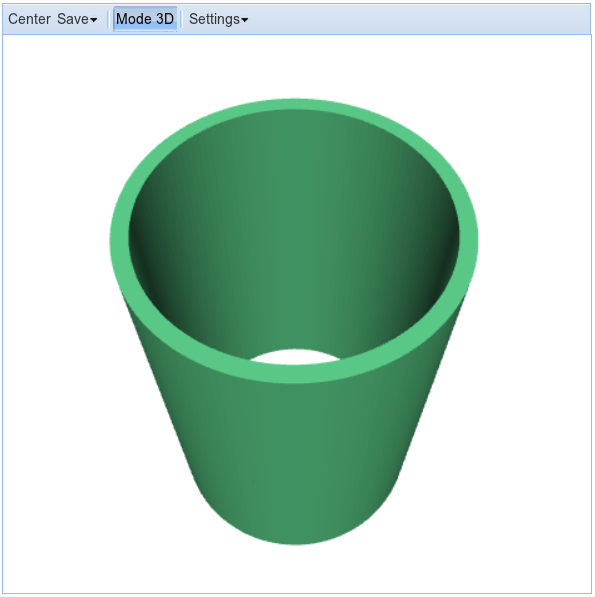
\includegraphics[width=0.5\textwidth]{img/tube-1.png}
\end{center}
\vspace{-2mm}
\caption{Tube of inner radius $r$, outer radius $R$ and height $H$.}
\label{fig:tube-1}
%\vspace{-1cm}
\end{figure}

\subsection{Command SPHERE}

A sphere of radius $R$ is rendered using the command SPHERE.
For example, the code

\begin{verbatim}
from pyplasm import *
R = 1.0
s = SPHERE(3.0)([64, 64])
lab.view(s, [0.4, 0.9, 0.6])
\end{verbatim}
will render a unit sphere whose origin is at (0, 0, 0). 
The parameter {\tt [64, 64]} stands for 
subdivision in both tangential directions. We need to be a bit 
careful with increasing this number, since doubling it to 
{\tt [128, 128]} would increase 
the number of linear faces approximation the sphere {\bf four times}.
The output of the above code is shown in Fig. \ref{fig:sphere-1}.

\newpage

\begin{figure}[!ht]
\begin{center}
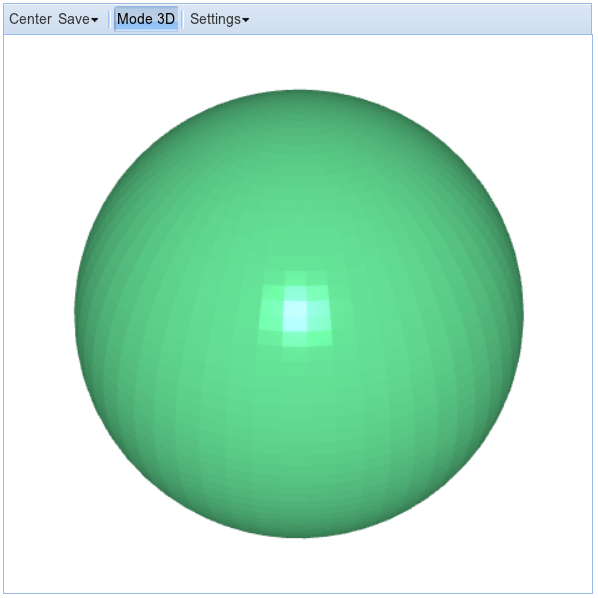
\includegraphics[width=0.5\textwidth]{img/sphere-1.png}
\end{center}
\vspace{-2mm}
\caption{Sphere of radius $R$ and origin (0, 0, 0).}
\label{fig:sphere-1}
%\vspace{-1cm}
\end{figure}


\subsection{Command TORUS}

The TORUS command takes an inner radius $r$ and outer radius 
$R$ as parameters. It is used as follows:
\begin{verbatim}
from pyplasm import *
r = 3.0
R = 5.0
tor = TORUS([r, R])([64, 64])
lab.view(tor, [0.4, 0.9, 0.6])
\end{verbatim}
The center of the torus is at the origin (0, 0, 0) and its axis
is the $z$-axis. This is illustrated in Fig. \ref{fig:torus-1}.

\newpage

\begin{figure}[!ht]
\begin{center}
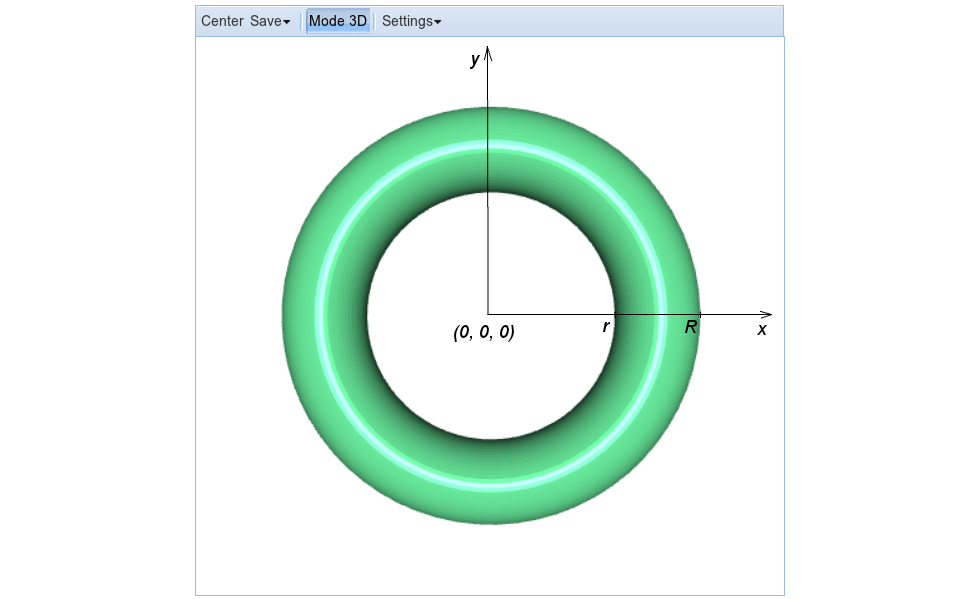
\includegraphics[width=0.82\textwidth]{img/torus-1.png}
\end{center}
\vspace{-2mm}
\caption{Torus of inner radius $r$, outer radius $R$ and center at the origin (0, 0, 0).}
\label{fig:torus-1}
%\vspace{-1cm}
\end{figure}

\subsection{Review questions}

\begin{enumerate}
\item Coming soon.
\begin{itemize}
\item[A1]
\item[A2]
\item[A3]
\item[A4]
\end{itemize}
\end{enumerate}


\subsection{Exercises}

\begin{enumerate}
\item
Create a $3 \times 4 \times 5$ brick in a light
blue color, as shown in Fig. \ref{fig:a1}.

\newpage

\begin{figure}[!ht]
\begin{center}
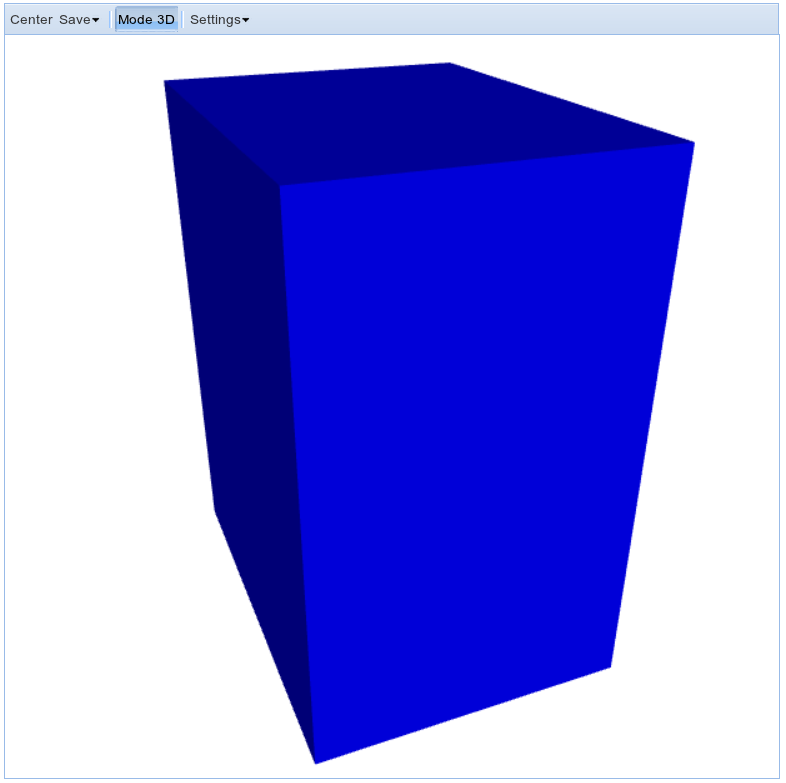
\includegraphics[width=0.5\textwidth]{img/a1-blue-brick.png}
\end{center}
\vspace{-2mm}
\caption{Illustration for Exercise 1.}
\label{fig:a1}
%\vspace{-1cm}
\end{figure}

\item Create a $3 \times 1$ rectangle in a light
red color, as shown in Fig. \ref{fig:a2}.

\begin{figure}[!ht]
\begin{center}

\includegraphics[width=0.5\textwidth]{img/a2-red-rectangle.png}
\end{center}
\vspace{-2mm}
\caption{Illustration for Exercise 2.}
\label{fig:a2}
\vspace{-0cm}
\end{figure}

\item Create an orange octahedron with vertices 
(0, -1, 1), (0, 1, 1), (0, -1, -1), (0, 1, -1), (2, 0, 0), and (-2, 0, 0), 
as shown in Fig. \ref{fig:a3}.

\begin{figure}[!ht]
\begin{center}
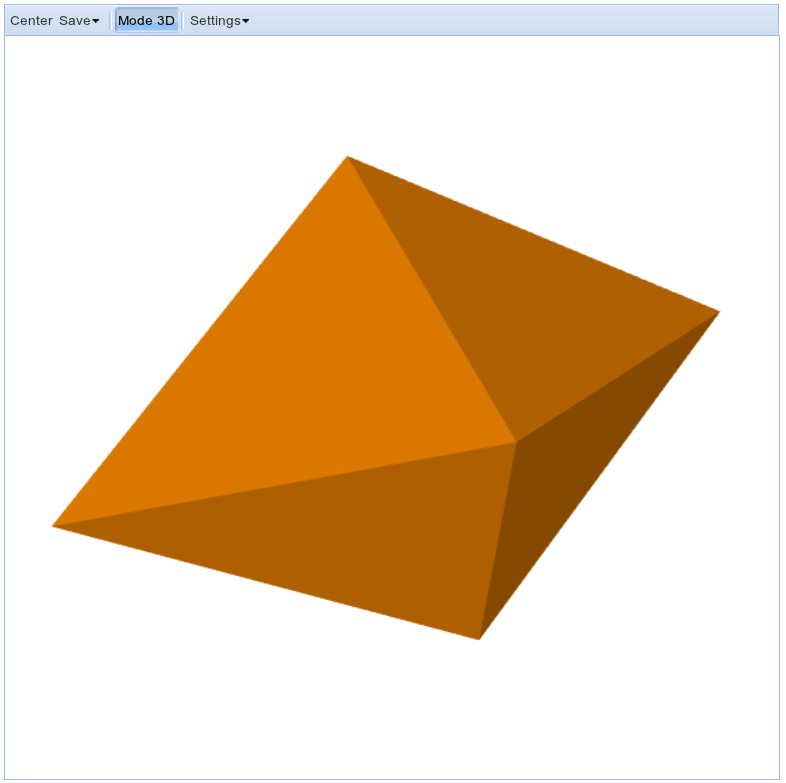
\includegraphics[width=0.5\textwidth]{img/a3-orange-octahedron.png}
\end{center}
\vspace{-2mm}
\caption{Illustration for Exercise 3.}
\label{fig:a3}
%\vspace{-1cm}
\end{figure}

\item Create a pink pentagon with equally-long edges that is inscribed 
in a circle with diameter $R$, as shown in Fig. \ref{fig:a4}.

\begin{figure}[!ht]
\begin{center}
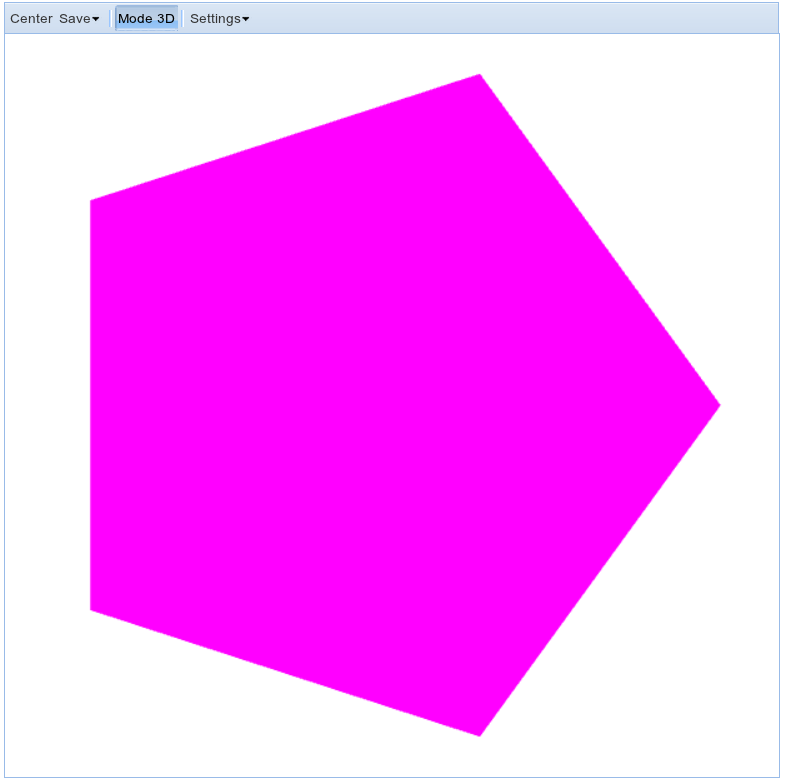
\includegraphics[width=0.5\textwidth]{img/a4-pink-pentagon.png}
\end{center}
\vspace{-4mm}
\caption{Illustration for Exercise 4.}
\label{fig:a4}
%\vspace{-4mm}
\end{figure}
\newpage

\item Create a cyan cone of radius $R$ and height $H$ that stands on its tip
(the tip is at (0, 0, 0) and the axis of the cone coincides with the 
$z$-axis), as shown in Fig. \ref{fig:a5}.

\begin{figure}[!ht]
\begin{center}
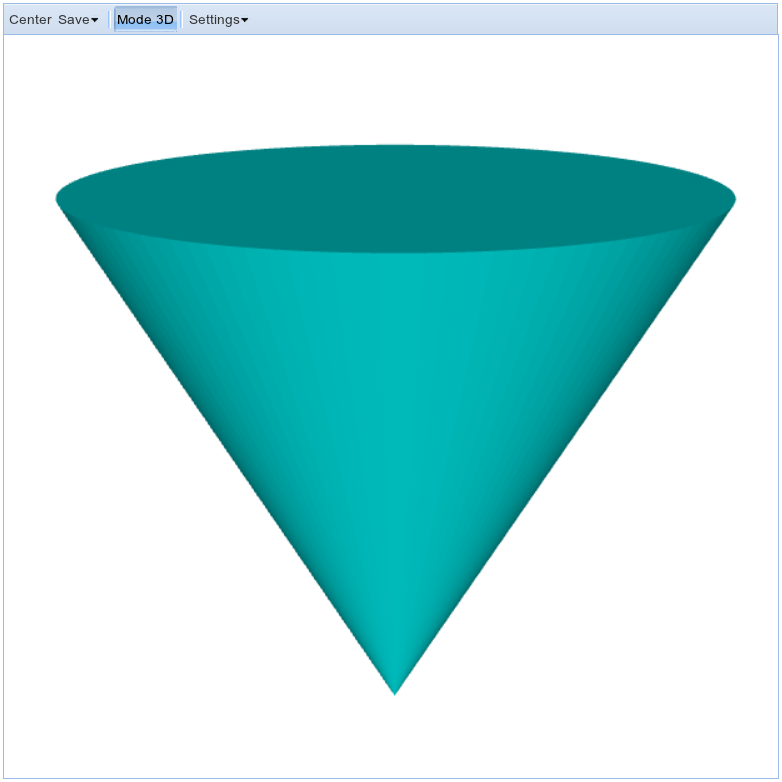
\includegraphics[width=0.5\textwidth]{img/a5-cyan-cone.png}
\end{center}
\vspace{-4mm}
\caption{Illustration for Exercise 5.}
\label{fig:a5}
%\vspace{-1cm}
\end{figure}

\item  Create a carmine cylinder of radius $R$ and height $H$, 
as shown in Fig. \ref{fig:a6}.

\begin{figure}[!ht]
\begin{center}
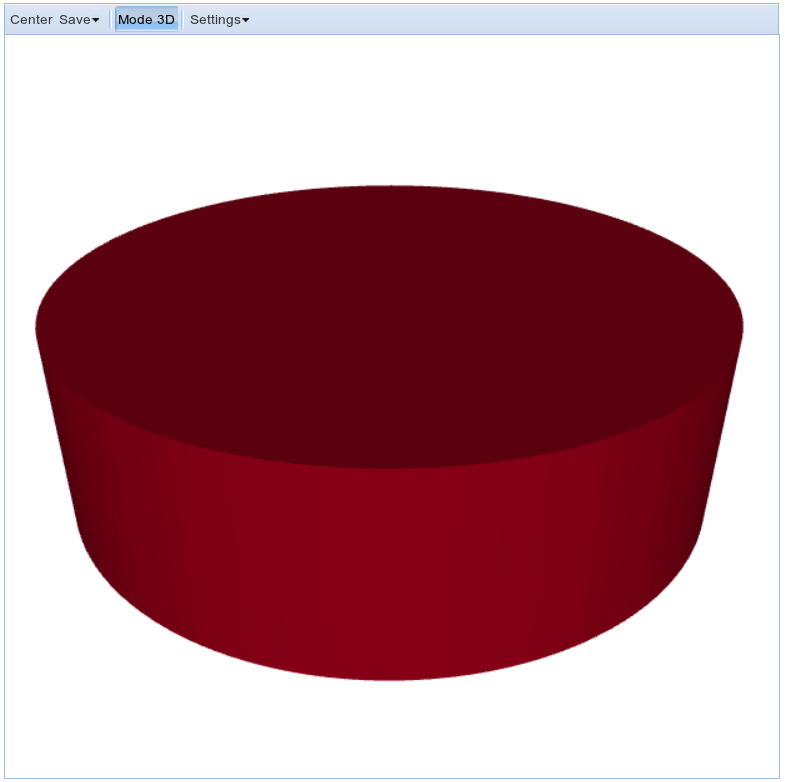
\includegraphics[width=0.5\textwidth]{img/a6-carmine-cylinder.png}
\end{center}
\vspace{-2mm}
\caption{Illustration for Exercise 6.}
\label{fig:a6}
%\vspace{-1cm}
\end{figure}
\newpage

\item Create a topaz tube of inner radius $R_{in}$, outer radius $R_{out}$
and height $H$, as shown in Fig. \ref{fig:a7}.


\begin{figure}[!ht]
\begin{center}
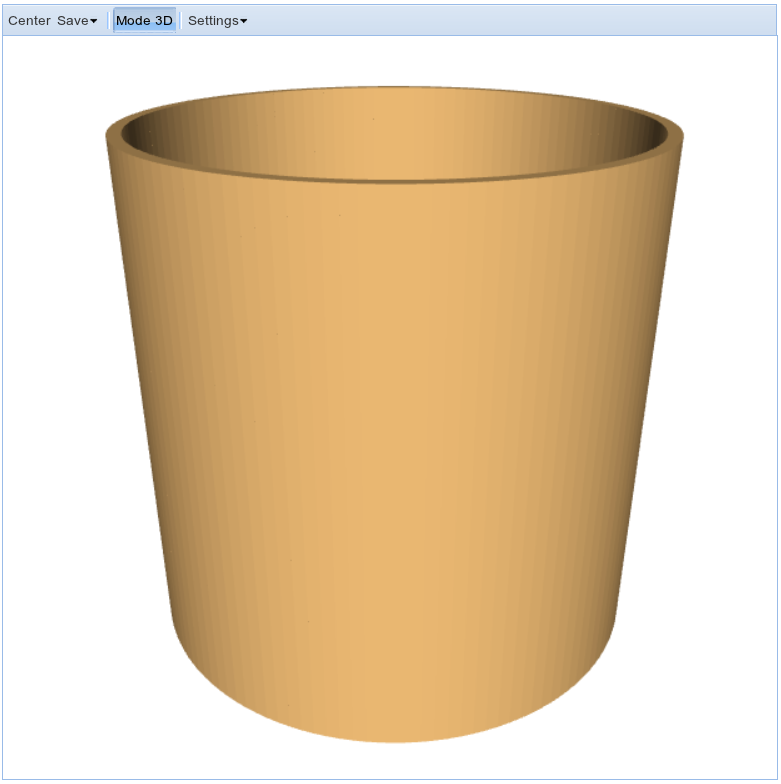
\includegraphics[width=0.5\textwidth]{img/a7-topaz-tube.png}
\end{center}
\vspace{-2mm}
\caption{Illustration for Exercise 7.}
\label{fig:a7}
%\vspace{-1cm}
\end{figure}

\item Create a sand sphere of radius $R$ and center at the origin (0, 0, 0). 
Use $[64, 64]$ for the piecewise-linear approximation of the curved surface, 
as shown in Fig. \ref{fig:a8}.


\begin{figure}[!ht]
\begin{center}
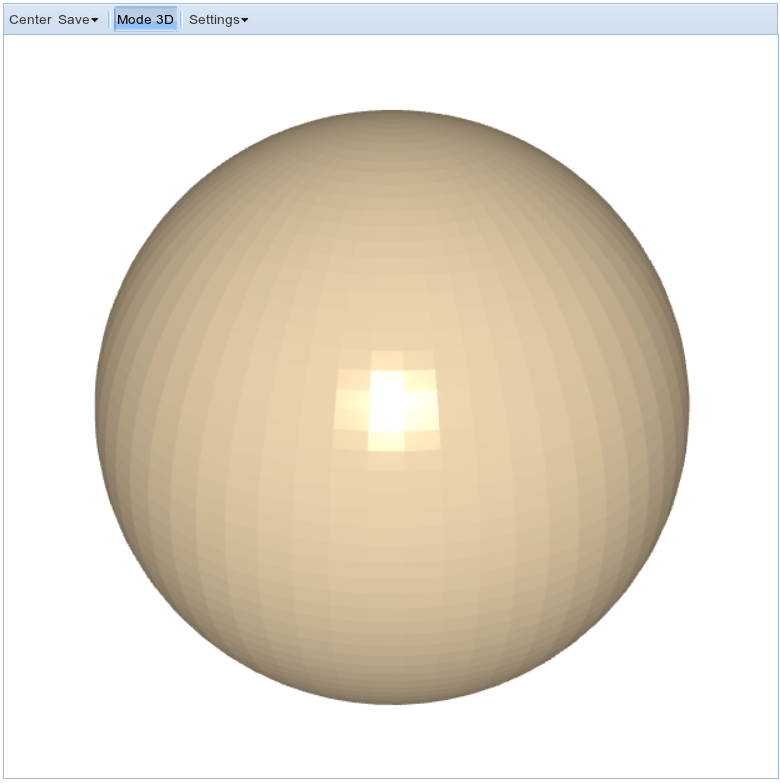
\includegraphics[width=0.5\textwidth]{img/a8-sand-sphere.png}
\end{center}
\vspace{-2mm}
\caption{Illustration for Exercise 8.}
\label{fig:a8}
\vspace{-1cm}
\end{figure}
\newpage

\item Create a turquoise torus of inner radius $R_{in}$ and outer radius $R_{out}$, whose center 
is at the origin (0, 0, 0). Use $[64, 64]$ for the piecewise-linear approximation 
of the curved surface, as shown in Fig. \ref{fig:a9}.


\begin{figure}[!ht]
\begin{center}
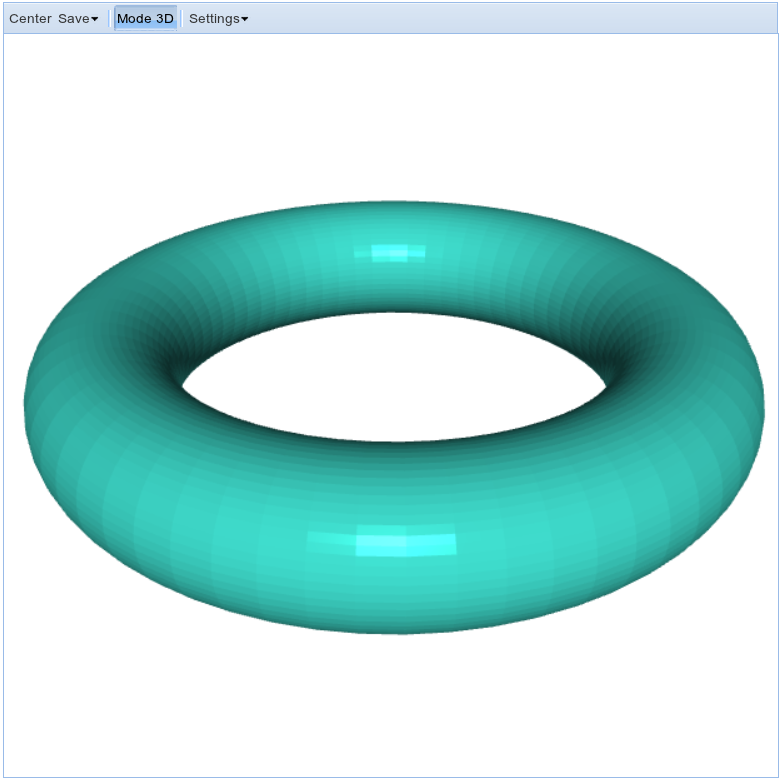
\includegraphics[width=0.5\textwidth]{img/a9-turquoise-torus.png}
\end{center}
\vspace{-2mm}
\caption{Illustration for Exercise 9.}
\label{fig:a9}
%\vspace{-1cm}
\end{figure}

\item Write a script to render a cylinder of radius {\tt R} and height {\tt H}
      via the CONVEXHULL command. The cylinder's axis should coincide with the 
      $z$-axis, the center of its base circle should be (0, 0, 0), and the 
      curved surface should be subdivided into {\tt subdiv} linear segments.

\end{enumerate}
\newpage

%%%%%%%%%%%%%%%%%%%%%%%%%%%%%%%%%%%%%%%%%%%%%%%%%%%%%%%%%%%%%%%%%%%%%%%%%%%%%%%
\iffullversion
\else
\vbox{}
\vfill
\pagestyle{empty}
    \begin{center}
    {\huge \color{red}END OF PREVIEW}\\[2cm]

\centerline{\Large Please consider:}
\vspace{1cm}

{\Large \bf Purchasing Online Course with Curriculum}
\vspace{1cm}

    {\Large or,}\\[1cm]

{\Large \bf Ordering Textbook and Solution Manual}
\vspace{1cm}

    {\Large For either, visit {\tt http://introtocad.net}. \\[2cm]
}
\end{center}
{\bf The course includes}:
\begin{itemize}
\item Access to full version of textbook and solution manual.
\item One-click download of interactive review question worksheets.
\item One-click download of interactive programming exercises (in preparation).
\item One-click distribution to students in your class.
\item One-click collection, automated grading, and progress monitoring (in preparation).
\item Access to all answers and solution designs.
\end{itemize}

\vfill
    \end{document}
\fi

%%%%%%%%%%%%%%%%%%%%%%%%%%%%%%%%%%%%%%%%%%%%%%%%%%%%%%%%%%%%%%%%%%%%%%%%%%%%%%%

\section{Basic Transformations}

\subsection{Objectives}
\begin{itemize}
\item Learn to scale, translate, and rotate objects.
\item Learn to create compound objects.
\item Learn to put objects on top of each other.
\end{itemize}
So far we have learned how to create a variety of simple 2D and 3D objects. 
The next step is to learn how to scale, rotate, and translate them. PLaSM
provides simple commands for that. Let us begin with scaling.

\subsection{Command SCALE}

The SCALE command takes three arguments: A list of axial directions in which 
the object will be scaled (as integers), list of scaling factors for these 
directions, and the object to be scaled. For example, let us create a cylinder 
{\tt cyl} of radius 1.0 and height 0.3:

\begin{verbatim}
from pyplasm import *
cyl = CYLINDER([1.0, 0.3])(128)
\end{verbatim}
We know from before that the axis of this cylinder coincides with the $z$-axis 
and that the center of its bottom face is at (0, 0, 0). The output is shown in Fig. \ref{fig:scale-0}.

\begin{figure}[!ht]
\begin{center}
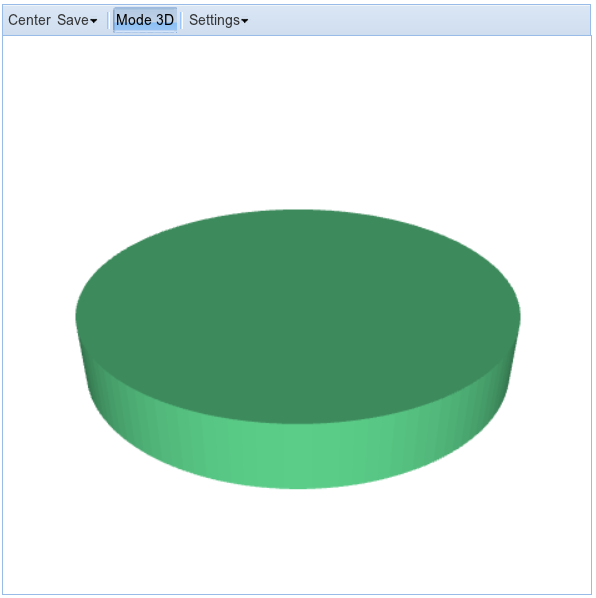
\includegraphics[width=0.5\textwidth]{img/scale-0.png}
\end{center}
\vspace{-2mm}
\caption{Cylinder of radius 1.0 and height 0.3.}
\label{fig:scale-0}
%\vspace{-1cm}
\end{figure}

\noindent
\underline{\em Scaling in $x$-direction}\\

The following command will 
scale the cylinder in the $x$-direction by the factor of 2.0: 

\begin{verbatim}
cyl1 = SCALE([1])([2.0])(cyl)
lab.view(cyl1, [0.4, 0.9, 0.6])
\end{verbatim}
In fact, the $x$-coordinate of all points forming 
the object will be multiplied by 2.0. So, the axis of the resulting object will still
coincide with the $z$-axis, and the center of its bottom face will
still be at the origin (0, 0, 0). Only its limits in the $x$-direction will change 
from (-1.0, 1.0) to (-2.0, 2.0).
The output is shown in Fig. \ref{fig:scale-1}.

\begin{figure}[!ht]
\begin{center}
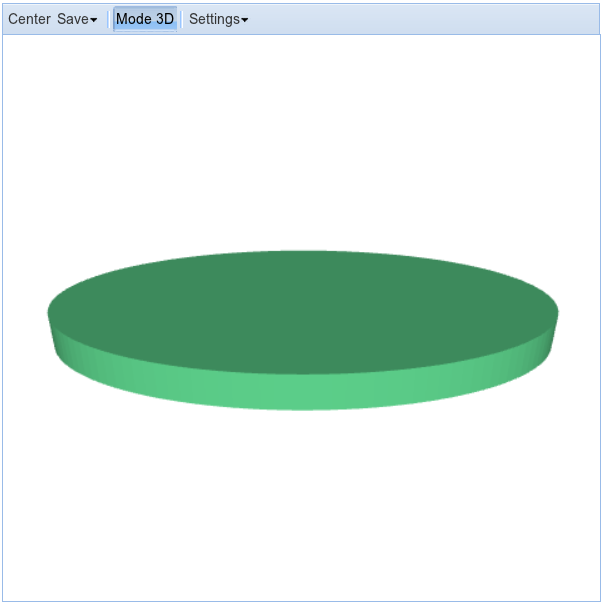
\includegraphics[width=0.5\textwidth]{img/scale-1.png}
\end{center}
\vspace{-2mm}
\caption{Cylinder scaled in the first axial direction by 2.0.}
\label{fig:scale-1}
%\vspace{-1cm}
\end{figure}

\noindent
\underline{\em Scaling in $y$-direction}\\

The following command will 
scale the cylinder in the $y$-direction by the factor of 2.0: 

\begin{verbatim}
cyl2 = SCALE([2])([2.0])(cyl)
lab.view(cyl2, [0.4, 0.9, 0.6])
\end{verbatim}
The axis of the resulting object will still
coincide with the $z$-axis, and the center of its bottom face will
still be at the origin (0, 0, 0). Only its limits in the $y$-direction will change 
from (-1.0, 1.0) to (-2.0, 2.0).
The output is shown in Fig. \ref{fig:scale-2}.

\newpage

\begin{figure}[!ht]
\begin{center}
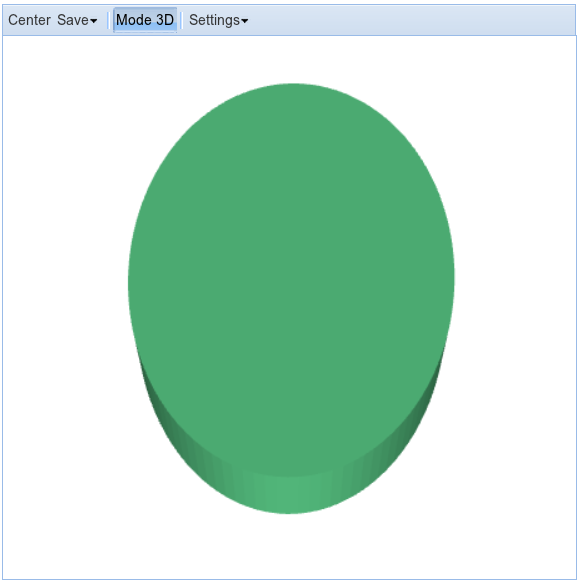
\includegraphics[width=0.5\textwidth]{img/scale-2.png}
\end{center}
\vspace{-2mm}
\caption{Cylinder scaled in the second axial direction by 2.0.}
\label{fig:scale-2}
%\vspace{-1cm}
\end{figure}

\noindent
\underline{\em Scaling in $z$-direction}\\

The following command will 
scale the cylinder in the $z$-direction by the factor of 2.0: 

\begin{verbatim}
cyl3 = SCALE([3])([2.0])(cyl)
lab.view(cyl3, [0.4, 0.9, 0.6])
\end{verbatim}
The axis of the resulting object will still
coincide with the $z$-axis, and the center of its bottom face will
still be at the origin (0, 0, 0). Only its limits in the $z$-direction will change 
from (0.0, 0.3) to (0.0, 0.6). The output is shown in Fig. \ref{fig:scale-3}.

\newpage

\begin{figure}[!ht]
\begin{center}
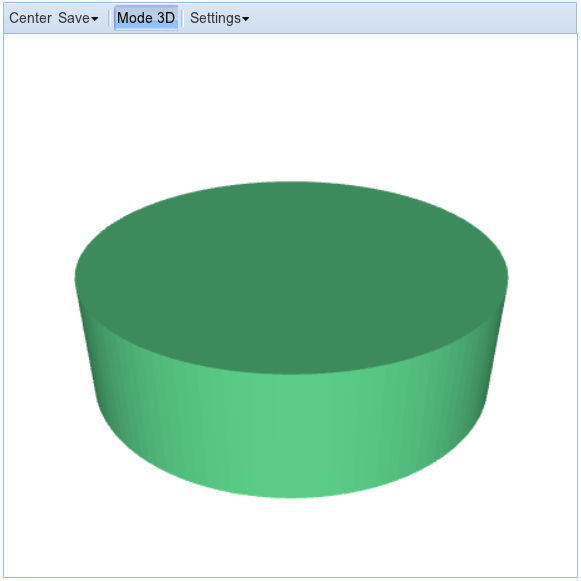
\includegraphics[width=0.5\textwidth]{img/scale-3.png}
\end{center}
\vspace{-2mm}
\caption{Cylinder scaled in the third axial direction by 2.0.}
\label{fig:scale-3}
%\vspace{-1cm}
\end{figure}

\noindent
\underline{\em Scaling in $x$ and $z$ directions simultaneously}\\

The following command will 
scale the cylinder simultaneously in the $x$- directions by 2.0 and in the $z$-direction by 4.0.
This can be viewed as scaling in the $xz$-plane:

\begin{verbatim}
cyl4 = SCALE([1, 3])([2.0, 4.0])(cyl)
lab.view(cyl4, [0.4, 0.9, 0.6])
\end{verbatim}
The axis of the resulting object will still
coincide with the $z$-axis, and the center of its bottom face will
still be at the origin (0, 0, 0). Only its limits in the $x$-direction 
will change from (-1.0, 1.0) to (-2.0, 2.0), and the limits in the 
$z$-direction will change 
from (0.0, 0.3) to (0.0, 1.2). The output is shown in Fig. \ref{fig:scale-4}.

\newpage

\begin{figure}[!ht]
\begin{center}
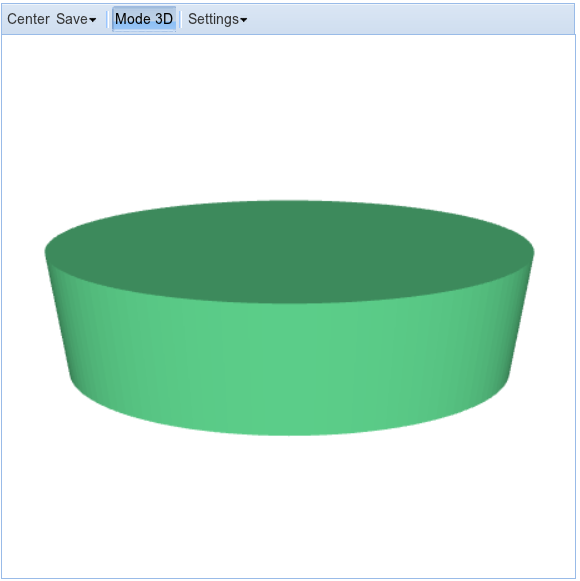
\includegraphics[width=0.5\textwidth]{img/scale-4.png}
\end{center}
\vspace{-2mm}
\caption{Cylinder scaled in the first and third axial directions by 2.0 and 4.0, respectively.}
\label{fig:scale-4}
%\vspace{-1cm}
\end{figure}
\noindent
Similarly, we could scale the object in the $xy$-plane using 

\begin{verbatim}
cyl4 = SCALE([1, 2])([2.0, 4.0])(cyl)
lab.view(cyl4, [0.4, 0.9, 0.6])
\end{verbatim}
or in the $yz$-plane using 

\begin{verbatim}
cyl4 = SCALE([2, 3])([2.0, 4.0])(cyl)
lab.view(cyl4, [0.4, 0.9, 0.6])
\end{verbatim}

\noindent
\underline{\em Scaling in all exial directions simultaneously}\\

The following command will 
scale the cylinder simultaneously in all three axial directions by the factors
2.0, 0.5 and 4.0.

\begin{verbatim}
cyl5 = SCALE([1, 2, 3])([2.0, 0.5, 4.0])(cyl)
lab.view(cyl5, [0.4, 0.9, 0.6])
\end{verbatim}
The output is shown in Fig. \ref{fig:scale-5}.

\newpage

\begin{figure}[!ht]
\begin{center}
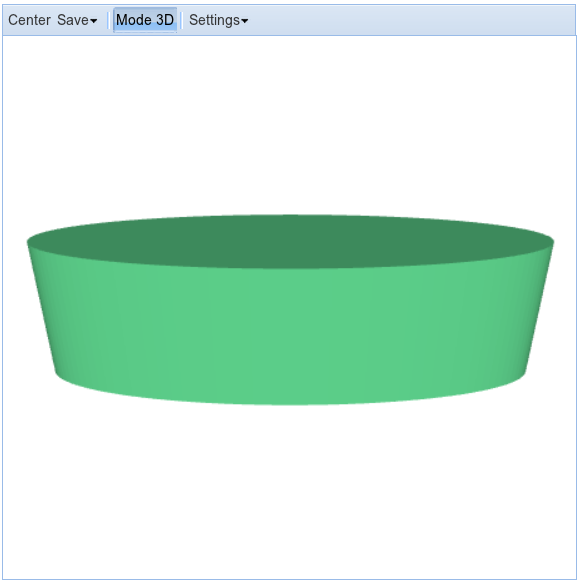
\includegraphics[width=0.5\textwidth]{img/scale-5.png}
\end{center}
\vspace{-2mm}
\caption{Cylinder scaled in all three axial directions simultaneously.}
\label{fig:scale-5}
%\vspace{-1cm}
\end{figure}
\noindent
We believe that the reader has now a good understanding of scaling.
In Section \ref{sec:translate} we will discuss in more detail how
to properly combine scaling with translations. 

\subsection{Enlarging an object}
If we want to just enlarge an object, we use the command SCALE and 
apply the same factor in all spatial directions. For example, to 
make a cylinder {\tt cyl} 5-times larger, we type:

\begin{verbatim}
cyl6 = SCALE([1, 2, 3])([5.0, 5.0, 5.0])(cyl)
lab.view(cyl6, [0.4, 0.9, 0.6])
\end{verbatim}


\subsection{Command TRANSLATE} \label{sec:translate}

The TRANSLATE command (abbreviated as T) can be used to move any 
object to a desired location. It takes three arguments: Axial directions,
displacements in these directions, and the object to be moved. For example,
the following program creates a unit cube and moves it by 1.5 in the 
$x$-direction:

\begin{verbatim}
from pyplasm import *
cube = CUBE(1.0)
cube2 = T(1)(1.5)(cube)
\end{verbatim}
Another example: We create a unit sphere and move it simultaneously 
in the $x$-direction by 1.0 and in the $y$-direction by 2.0:

\begin{verbatim}
from pyplasm import *
s = SPHERE(1.0)([64, 64])
s2 = T([1, 2])([1.0, 2.0])(s)
\end{verbatim}
And last example: We create a unit sphere and  
move it simultaneously by -1.0 in the $x$-direction, by 1.0 in the $y$-direction
and by 4.0 in the $z$-direction:

\begin{verbatim}
from pyplasm import *
s = SPHERE(1.0)([64, 64])
s2 = T([1, 2, 3])([-1.0, 1.0, 4.0])(s)
\end{verbatim}

\subsection{Compound objects - command STRUCT}

Creating compound objects is necessary
for plotting multiple objects, since {\tt lab.view()} only can 
display a single object. This is also practical 
when we need to scale, translate, or rotate multiple objects at
once. For example, let's create a cube with a sphere on top of it.
It is always important to remember how a newly created
object is positioned in the global coordinate system. Concretely,
recall that {\tt CUBE} and {\tt CUBOID} are aligned with the 
axes as shown in Fig. \ref{fig:cuboid-1}

\begin{verbatim}
from pyplasm import *
color = [0.9, 0.9, 0.9]
c = CUBE(2.0)
c2 = T([1, 2, 3])([1.0, 1.0, 2.0])(c)
c3 = T([1, 2, 3])([1.0, 1.0, 2.0])(c2)
\end{verbatim}
The way to display the three cubes together
is to create a compound object containing all of them:

\begin{verbatim}
comp = STRUCT([c, c2, c3])
lab.view(comp, [0.4, 0.9, 0.6])
\end{verbatim}
The output is shown in Fig. \ref{fig:comp-1}

\newpage

\begin{figure}[!ht]
\begin{center}
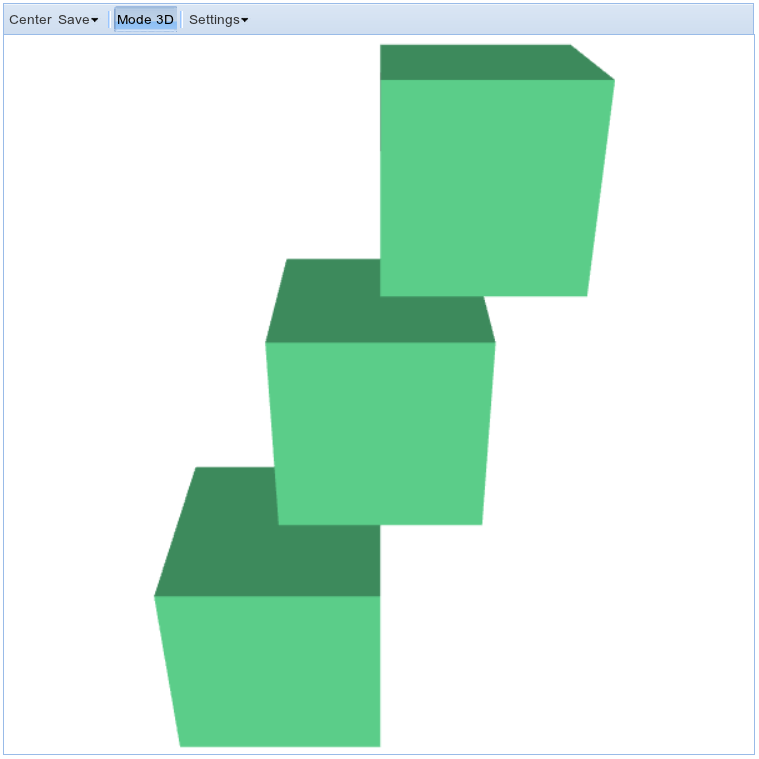
\includegraphics[width=0.5\textwidth]{img/comp-1.png}
\end{center}
\vspace{-2mm}
\caption{The way to display all cubes together is to use the STRUCT command.}
\label{fig:comp-1}
%\vspace{-1cm}
\end{figure}


\subsection{Putting objects on top of each other - command TOP}

The TOP command is a special case of translation that is very 
useful when we need to put objects on top of each other.
For illustration, let us put a sphere on top of a cube:

\begin{verbatim}
from pyplasm import *
c = CUBE(2.0)
s = SPHERE(1.0)([64, 64])
lab.view(TOP([c, s]), color)
\end{verbatim}
The output is shown in Fig. \ref{fig:top-1}:

\newpage

\begin{figure}[!ht]
\begin{center}
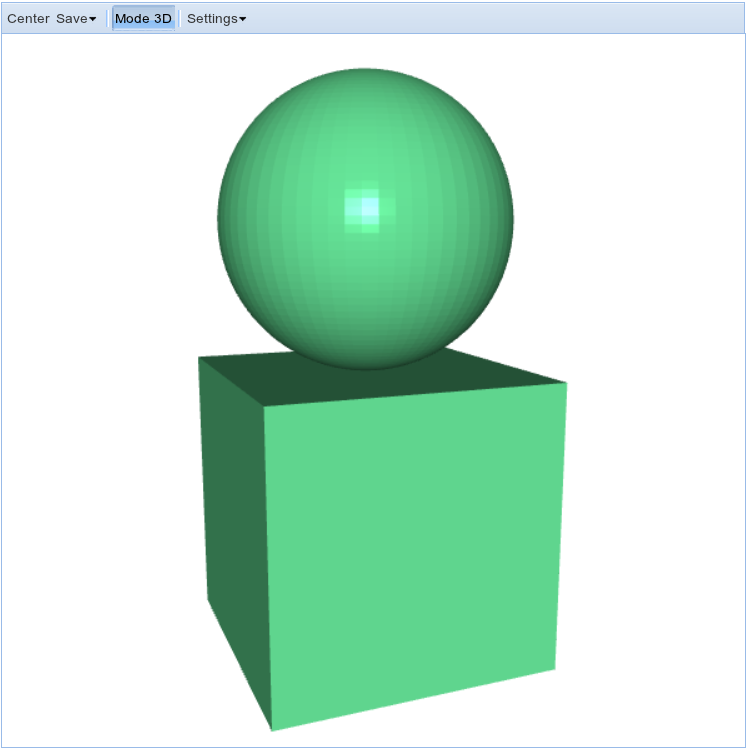
\includegraphics[width=0.5\textwidth]{img/top-1.png}
\end{center}
\vspace{-2mm}
\caption{Putting a sphere on top of a cube.}
\label{fig:top-1}
%\vspace{-1cm}
\end{figure}



\subsection{Command ROTATE}

Objects can be rotated using the command ROTATE (that
can be abbreviated as R). It has three parameters:
A pair of axes defining the plane of rotation (as integers),
an angle, and the object to be rotated. The axis of rotation 
always passes through the origin (0, 0, 0), so it is important 
to know exactly where your object is located. 

For example, when creating 
a CUBOID, it is positioned as shown in Fig. \ref{fig:cuboid-1}.
Hence, the axis of rotation does not pass through its center!
This is best illustrated using a simple example. Let us create 
a unit cube, rotate it by $\pi$ (180 degrees), and display 
the rotated cube together with the original one:

\begin{verbatim}
from pyplasm import *
cube = CUBE(1.0)
cube2 = R([1, 2])(PI)(cube)
comp = STRUCT([cube, cube2])
lab.view(comp, [0.4, 0.9, 0.6])
\end{verbatim}
The output is shown in Fig. \ref{fig:rot-1}.

\newpage

\begin{figure}[!ht]
\begin{center}
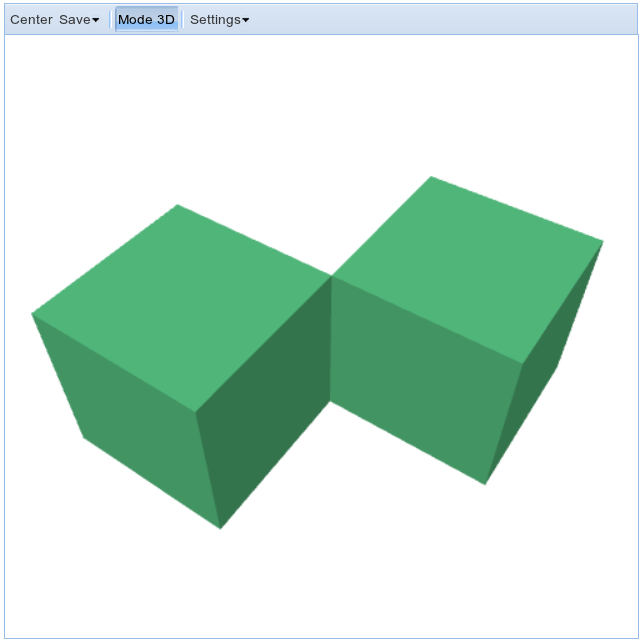
\includegraphics[width=0.5\textwidth]{img/rot-1.png}
\end{center}
\vspace{-2mm}
\caption{Unit cube rotated by $\pi$ (180 degrees) shown together with the original unit cube.}
\label{fig:rot-1}
%\vspace{-1cm}
\end{figure}
\noindent
In Fig. \ref{fig:rot-1}, the axis of rotation is where the two cubes meet. 

If we wanted to 
rotate the cube "in place", so that its center would not be moved,
we would have to first translate the cube in such a way that its center
lies at the origin. Let's do this. After moving the cube so that 
its center is at (0, 0, 0), we will rotate it in two different directions,
then move it by 2.0 in the $x$-direction and display along with 
the original cube for comparison:

\begin{verbatim}
from pyplasm import *
color = [0.4, 0.9, 0.6]
cube = CUBE(1.0)
cube2 = R([1, 2])(PI/4)(cube)
cube2 = R([2, 3])(PI/4)(cube2)
cube2 = T([1, 2, 3])([1, 1, 1])(cube2)

comp = STRUCT([cube, cube2])
lab.view(comp, color)
\end{verbatim}
The output is shown in Fig. \ref{fig:rot-2}.
\newpage

\begin{figure}[!ht]
\begin{center}
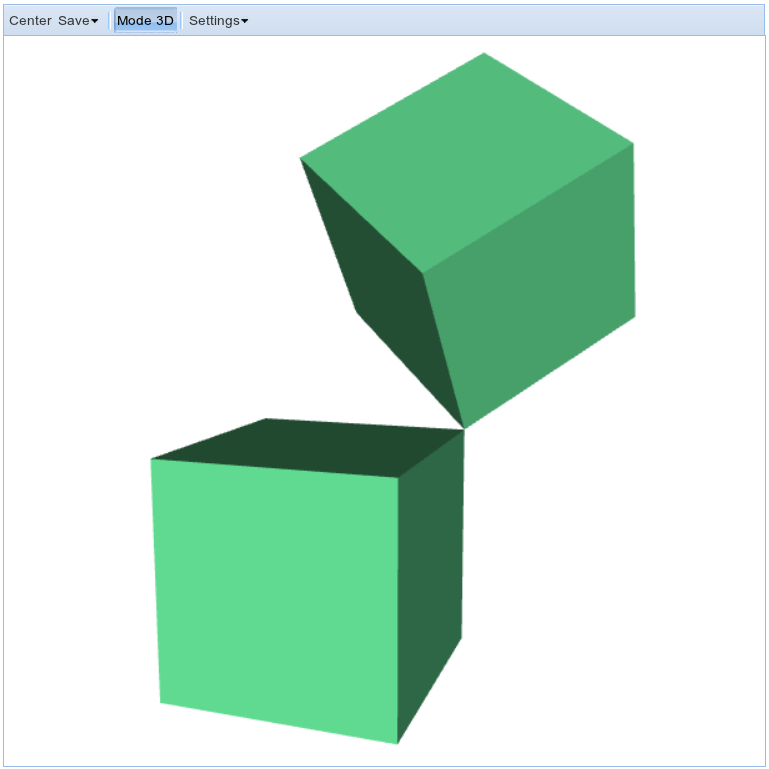
\includegraphics[width=0.5\textwidth]{img/rot-2.png}
\end{center}
\vspace{-2mm}
\caption{Cube rotated in two directions, then moved and shown along with the original cube.}
\label{fig:rot-2}
%\vspace{-1cm}
\end{figure}

\subsection{Review questions}

\begin{enumerate}
\item Coming soon.
\begin{itemize}
\item[A1]
\item[A2]
\item[A3]
\item[A4]
\end{itemize}
\end{enumerate}

\subsection{Exercises}

\begin{enumerate}
\item 
Create a kitchen table shown in Fig. \ref{fig:b1}. All of its measures should be variable.

\newpage

\begin{figure}[!ht]
\begin{center}
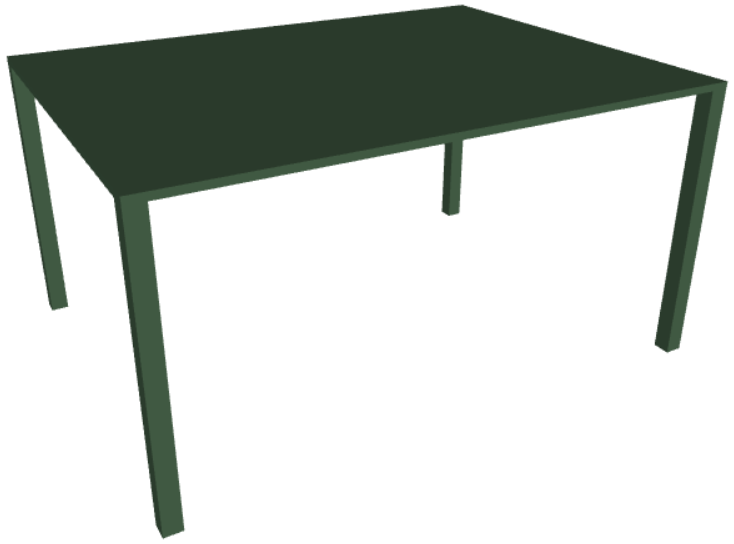
\includegraphics[width=0.5\textwidth]{img/kitchentable.png}
\end{center}
\vspace{-2mm}
\caption{Illustration for Exercise 1.}
\label{fig:b1}
%\vspace{-1cm}
\end{figure}

\item Create a round tea table with round legs as
shown in Fig. \ref{fig:b2}. All of its measures should be variable.

\begin{figure}[!ht]
\begin{center}
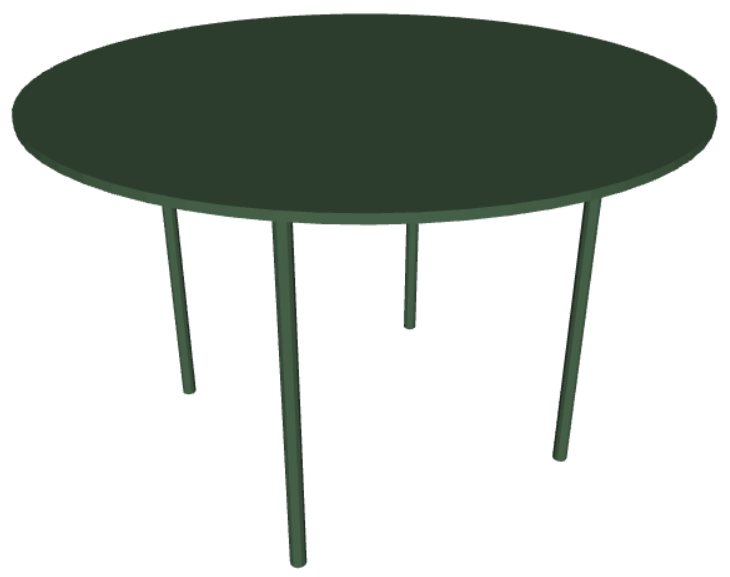
\includegraphics[width=0.5\textwidth]{img/teatable.png}
\end{center}
\vspace{-2mm}
\caption{Illustration for Exercise 2.}
\label{fig:b2}
%\vspace{-1cm}
\end{figure}

\item Use a scaled cylinder and a torus to create a padlock that is shown in Fig. \ref{fig:b3}. 
All of its measures should be variable.

\newpage

\begin{figure}[!ht]
\begin{center}
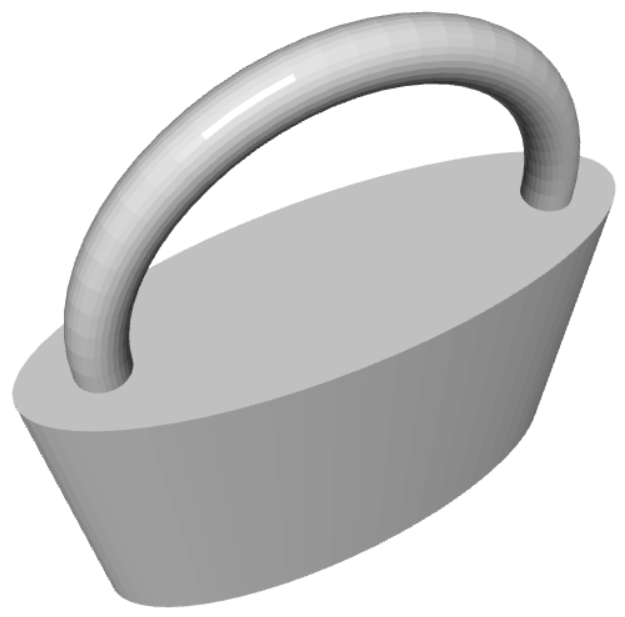
\includegraphics[width=0.4\textwidth]{img/padlock.png}
\end{center}
\vspace{-2mm}
\caption{Illustration for Exercise 3.}
\label{fig:b3}
%\vspace{-1cm}
\end{figure}

\item Use two cylinders and a sphere to create a bottle shown in Fig. \ref{fig:b4}. 
All of its measures should be variable.

\begin{figure}[!ht]
\begin{center}

\includegraphics[width=0.8\textwidth]{img/bottle.png}
\end{center}
\vspace{-2mm}
\caption{Illustration for Exercise 4.}
\label{fig:b4}
%\vspace{-1cm}
\end{figure}

\end{enumerate}

\section{Boolean Operations}

\subsection{Objectives}
\begin{itemize}
\item Understand why we do Boolean operations in Solid Modeling.
\item Learn how to subtract objects.
\item Learn to convert surfaces into solids.
\item Create union and intersection of objects.
\item Create exclusive or (xor) of objects.
\item Understand that Boolean operation should be done between as simple
      objects as possible. 
\end{itemize}
Boolean operations with objects are where things start to be real 
fun. Let us begin with the 
command DIFF that makes it possible to drill holes, cut and slice objects, 
round edges, make imprints, and much more.

\subsection{Subtracting objects -- command DIFF}

The command DIFF makes it possible to subtract one object from another.
For illustration, we will create a $2 \times 2 \times 2$ cube and subtract 
a cylinder of radius 1.5 from it. It is important to remember where in the 
coordinate system the objects are created -- the cube lies in the 
first quadrant, with three of its edges meeting at the origin (0, 0, 0).
The cylinder's axis coincides with the $z$-axis and the center of its base
circle is the origin. 

\begin{verbatim}
from pyplasm import *
c = CUBE(2.0)
s = CYLINDER([1.5, 2])(128)
lab.view(DIFF([c, s]), [0.4, 0.9, 0.6]) 
\end{verbatim}
The output is shown in Fig. \ref{fig:diff-1}.

\begin{figure}[!ht]
\begin{center}
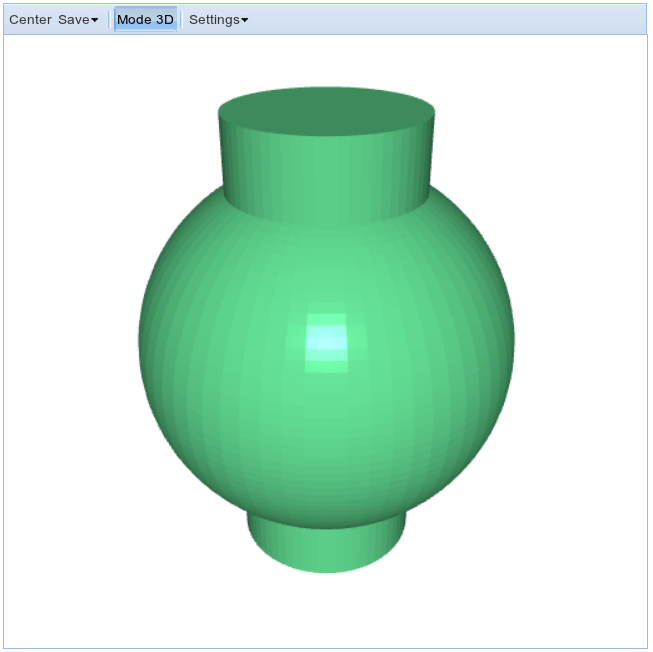
\includegraphics[width=0.5\textwidth]{img/diff-1.png}
\end{center}
\vspace{-2mm}
\caption{Subtracting the cylinder from the cube.}
\label{fig:diff-1}
%\vspace{-1cm}
\end{figure}
\noindent
We can also subtract the cube from the cylinder:

\begin{verbatim}
lab.view(DIFF([s, c]), [0.4, 0.9, 0.6]) 
\end{verbatim}
The output is shown in Fig. \ref{fig:diff-2}.

\newpage

\begin{figure}[!ht]
\begin{center}
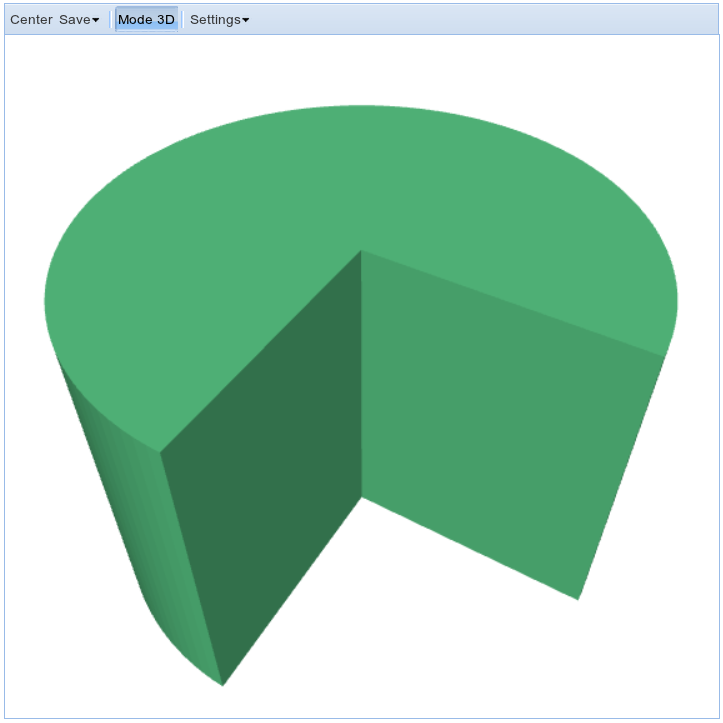
\includegraphics[width=0.5\textwidth]{img/diff-2.png}
\end{center}
\vspace{-2mm}
\caption{Subtracting the cube from the cylinder.}
\label{fig:diff-2}
%\vspace{-1cm}
\end{figure}
\noindent

\subsection{Surfaces and solids -- command JOIN} \label{par:join}

Some objects are solids (CUBE, CUBOID, SPHERE) while others are surfaces (SPHERE, TORUS). 
Attempting to perform any Boolean operation (DIFF, UNION, INTERSECTION, ...) between
a solid and a surface will result into an error. This can be circumvented by 
converting the surface into a solid first, using the command JOIN. For example,
the following program will not work:

\begin{verbatim}
from pyplasm import *
c = CUBE(2.0)
s = SPHERE(1.5)([64, 64])
lab.view(DIFF([c, s]), [0.9, 0.9, 0.9])
\end{verbatim}
but this program is correct:

\begin{verbatim}
from pyplasm import *
c = CUBE(2.0)
s = JOIN(SPHERE(1.5)([64, 64]))
lab.view(DIFF([c, s]), [0.9, 0.9, 0.9])
\end{verbatim}




\subsection{Command UNION}

The UNION command creates a new object that is the set union 
of two or more objects. For simplicity, let us use the same objects
as in the previous example. 

\begin{verbatim}
from pyplasm import *
c = CUBE(2.0)
s = CYLINDER([1.5, 2])(128)
lab.view(UNION([c, s]), [0.4, 0.9, 0.6]) 
\end{verbatim}
The output is shown in Fig. \ref{fig:union}.

%\newpage

\begin{figure}[!ht]
\begin{center}
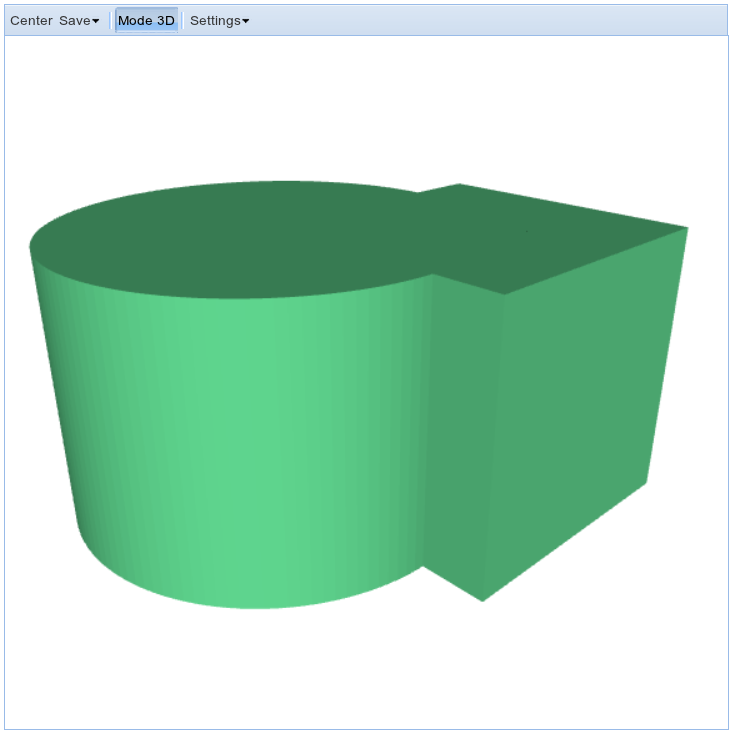
\includegraphics[width=0.5\textwidth]{img/union.png}
\end{center}
\vspace{-2mm}
\caption{Union of the cylinder and the cube.}
\label{fig:union}
%\vspace{-1cm}
\end{figure}


\subsection{Command INTERSECTION}

We will do two examples. First, for simplicity, we will create the intersection
of the cube and the cylinder from the previous paragraph:
 
\begin{verbatim}
from pyplasm import *
c = CUBE(2.0)
s = CYLINDER([1.5, 2])(128)
lab.view(INTERSECTION([c, s]), [0.4, 0.9, 0.6]) 
\end{verbatim}
The output is shown in Fig. \ref{fig:int-2}.

\newpage

\begin{figure}[!ht]
\begin{center}
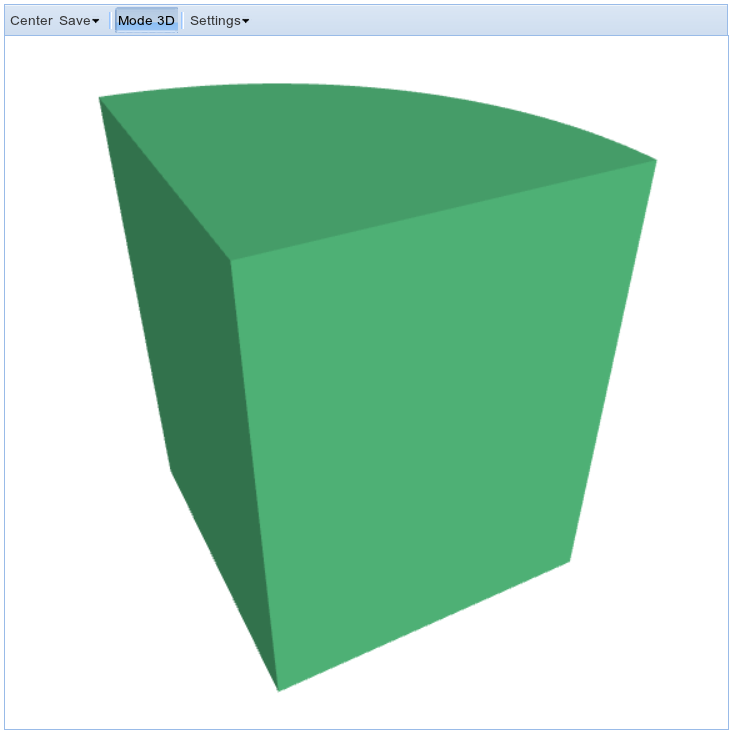
\includegraphics[width=0.5\textwidth]{img/int-2.png}
\end{center}
\vspace{-2mm}
\caption{Intersection of the cylinder and the cube.}
\label{fig:int-2}
%\vspace{-1cm}
\end{figure}
\noindent
In the second example, we will use the INTERSECTION command to create 
a strange object that looks link a square when viewed
from one direction, like a circle when viewed from another direction, 
and as a triangle when viewed from the third direction!


\begin{verbatim}
from pyplasm import *
color = [0.4, 0.9, 0.6]

# Cube.
c = CUBE(2.0)
c = T([1, 2, 3])([-1, -1, -1])(c)

# Cylinder.
cyl = CYLINDER([1, 2])(64)
cyl = T([3])([-1])(cyl)

# Prism.
p = CONVEXHULL([[1, -1, -1], [1, 0, 1], [1, 1, -1], \
[-1, -1, -1], [-1, 0, 1], [-1, 1, -1]])

# Show their intersection.
lab.view(INTERSECTION([c, cyl, p]), color)
\end{verbatim}
The output is shown in Fig. \ref{fig:diff-1}.

\begin{figure}[!ht]
\begin{center}

\includegraphics[width=0.25\textwidth]{img/int-1a.png}
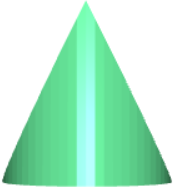
\includegraphics[width=0.25\textwidth]{img/int-1b.png}

\includegraphics[width=0.25\textwidth]{img/int-1c.png}
\end{center}
\vspace{-2mm}
\caption{Strange object!}
\label{fig:int-1}
%\vspace{-1cm}
\end{figure}


\subsection{Command XOR}

The operation XOR (exclusive logical OR) is "union minus intersection". Let us illustrate it 
on an example where we create a cube, and move it so that its center lies on the $z$-axis. Then 
we create a second cube by rotating the original cube by 45 degrees in the $xy$-plane. Last,
we XOR the two cubes. The corresponding code reads:
 
\begin{verbatim}
from pyplasm import *
color = [0.9, 0.9, 0.9]
c = CUBE(2.0)
c = T([1, 2])([-1, -1])(c)
c2 = R([1, 2])(PI/4.)(c)
lab.view(XOR([c, c2]), color) 
\end{verbatim}
The output is shown in Fig. \ref{fig:xor-1}.

\newpage

\begin{figure}[!ht]
\begin{center}
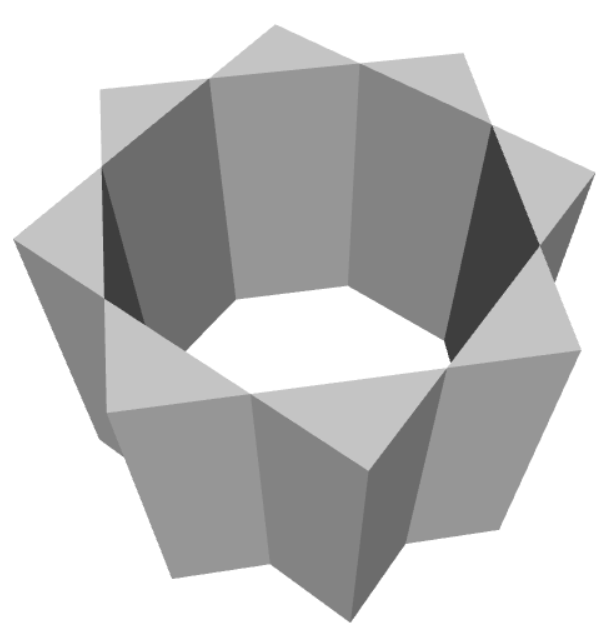
\includegraphics[width=0.5\textwidth]{img/xor-1.png}
\end{center}
\vspace{-2mm}
\caption{XOR of two overlapping cubes.}
\label{fig:xor-1}
%\vspace{-1cm}
\end{figure}
\noindent

\subsection{Doing it the wrong way, doing it the right way}

Boolean operations should be as much {\em local} as possible. This means
that they should occur between as {\em geometrically simple objects} as possible. If we 
ignore this rule, our computation times will be unnecessarily long and sometimes
we may hit a timeout in NCLab. 

We will demonstrate this on an example where we first create a vault and then play 
a gangster and drill a hole in it. Do not worry about the lenght of the script below  because
the vault has many small parts. But the fact that there are many parts is important here.
The model is available as Displayed Project "PLaSM - Examples - Vault". First, let us define the vault. 

{\small
\begin{verbatim}
# Import Plasm and define color:
from pyplasm import *
color = [200/255., 200/255., 200/255.]

# Define main vault body:
body = CUBOID([1, 1, 1.2])
interior = CUBOID([0.86, 0.95, 1.06])
interior = T([1, 2, 3])([0.07, 0, 0.07])(interior)
body = DIFF([body, interior])

# Top part:
top = CONVEXHULL([[0, 0, 1.2], [1, 0, 1.2], [1, 1, 1.2], [0, 1, 1.2], [0.01, 0.01, 1.21], 
[0.99, 0.01, 1.21], [0.99, 0.99, 1.21], [0.01, 0.99, 1.12]   ])

# Shelves:
shelf = CUBOID([1, 0.85, 0.02])
shelf1 = T([2, 3])([0.1, 0.4])(shelf)
shelf2 = T([3])([0.4])(shelf1)

# Front door:
door = CUBOID([0.84, 0.05, 1.04])
door = T([1, 2, 3])([0.08, 0, 0.08])(door)
door_frame = CUBOID([0.86, 0.03, 1.06])
door_frame = T([1, 2, 3])([0.07, 0.02, 0.07])(door_frame)

# Truncated cone under the handles:
tcone = JOIN(TRUNCONE([0.14, 0.13, 0.02])(64))
tcone = R([2, 3])(PI/2)(tcone)
tcone = T([1, 3])([0.5, 0.6])(tcone)

# Cylinder that holds the handles:
cyl = CYLINDER([0.07, 0.1])(64)
cyl = R([2, 3])(PI/2)(cyl)
cyl = T([1, 3])([0.5, 0.6])(cyl)

# Small truncated cone at the handles:
stcone = JOIN(TRUNCONE([0.07, 0.06, 0.01])(64))
stcone = R([2, 3])(PI/2)(stcone)
stcone = T([1, 2, 3])([0.5, -0.1, 0.6])(stcone)

# Handles:
h1 = CYLINDER([0.022, 0.3])(32)
ts = JOIN(TRUNCONE([0.022, 0.017, 0.01])(32))
ts = T([3])([0.3])(ts)
h1 = UNION([h1, ts])
h1 = R([2, 3])(PI/24)(h1)
h1 = R([1, 3])(-7*PI/24)(h1)
h2 = R([1, 3])(-2*PI/3)(h1)
h3 = R([1, 3])(-2*PI/3)(h2)
h1 = T([1, 2, 3])([0.5, -0.06, 0.6])(h1)
h2 = T([1, 2, 3])([0.5, -0.06, 0.6])(h2)
h3 = T([1, 2, 3])([0.5, -0.06, 0.6])(h3)

# Bolts:
b1 = CONVEXHULL([[0.81, 0, 0.19], [0.83, 0, 0.17], [0.97, 0, 0.17], [0.97, 0, 0.26], 
[0.83, 0, 0.26], [0.81, 0, 0.24], [0.815, -0.01, 0.195], [0.835, -0.01, 0.175], 
[0.965, -0.01, 0.175], [0.965, -0.01, 0.255], [0.835, -0.01, 0.255], [0.815, -0.01, 0.235]])
b2 = T([3])([0.77])(b1)

# Bolt cylinder:
bc = CYLINDER([0.015, 0.1])(16)
bc1 = T([1, 2, 3])([0.925, -0.009, 0.165])(bc)
bc2 = T([3])([0.77])(bc1)

# Small bolt sphere:
sbc = JOIN(SPHERE(0.01)([8, 8]))
sbc = R([2, 3])(PI/2)(sbc)
sbc1 = T([1, 2, 3])([0.845, -0.01, 0.195])(sbc)
sbc2 = T([3])([0.035])(sbc1)
sbc3 = T([3])([0.77])(sbc1)
sbc4 = T([3])([0.035])(sbc3)

# Vertical handle:
vh = CYLINDER([0.02, 0.5])(16)
vh = T([1, 2, 3])([0.15, -0.04, 0.35])(vh)

# Vertical handle supports:
vh0 = CYLINDER([0.015, 0.06])(16)
vh0 = R([2, 3])(PI/2)(vh0)
vh0 = T([1, 2, 3])([0.15, 0.02, 0.4])(vh0)
vh1 = T([3])([0.4])(vh0)

# Put everything together:
rest = STRUCT([top, shelf1, shelf2, door, door_frame, tcone, cyl, stcone, h1, h2, h3, b1, 
b2, bc1, bc2, sbc1, sbc2, sbc3, sbc4, vh, vh0, vh1])
vault = STRUCT([body, rest])
lab.view(vault, color)
\end{verbatim}
}
\noindent
The output is shown in Fig.\ref{fig:vault}.

\begin{figure}[!ht]
\begin{center}
\includegraphics[width=0.4\textwidth]{img/vault.png}
\end{center}
\vspace{-2mm}
\caption{Vault model.}
\label{fig:vault}
%\vspace{-1cm}
\end{figure}
\noindent
Now let's define a drill (3D cylinder): 
\begin{verbatim}
drill = CYLINDER([0.1, 0.5])(64)
drill = R([1, 3])(PI/2)(drill)
drill = T([1, 2, 3])([0.1, 0.5, 0.55])(drill)
\end{verbatim}
Now let's drill into the vault (subtract the cylinder from the vault). First we will do it 
the wrong way -- drilling into the {\tt vault} object. This is not smart because 
the {\tt vault} object consists of many different parts.

\begin{verbatim}
drilled_vault = DIFF([vault, drill])
lab.view(STRUCT([drilled_vault]), color)
\end{verbatim}
You can run this script but it will take a huge amount of time!

Instead, let us do it correctly -- we will perform the Boolean operation between the {\tt drill}
and the {\tt body} because {\tt body} is much geometrically simpler than {\tt vault}. Then
we will display the drilled body along with the rest of the vault. 

\begin{verbatim}
drilled_body = DIFF([body, drill])
lab.view(STRUCT([drilled_body, rest]), color)
\end{verbatim}
Note that the many small parts 
forming the object {\tt rest} are now not part of the Boolean 
operation at all, which makes it much simpler and faster.
The output is shown in Fig.\ref{fig:vault2}.


\begin{figure}[!ht]
\begin{center}
\includegraphics[width=0.4\textwidth]{img/vault2.png}
\end{center}
\vspace{-2mm}
\caption{Vault is drilled, and money is gone!}
\label{fig:vault2}
\end{figure}
\noindent

\subsection{Review questions}

\begin{enumerate}
\item Coming soon.
\begin{itemize}
\item[A1]
\item[A2]
\item[A3]
\item[A4]
\end{itemize}
\end{enumerate}

\subsection{Exercises}

\begin{enumerate}

\item Use a $4 \times 4 \times 4$ brick to create the object shown in 
Fig. \ref{fig:nclabicon}.

\newpage

\begin{figure}[!ht]
\begin{center}
\includegraphics[width=0.5\textwidth]{img/nclabicon.png}
\end{center}
\vspace{-2mm}
\caption{Illustration for Exercise 1.}
\label{fig:nclabicon}
%\vspace{-1cm}
\end{figure}
\noindent

\item Create a cube and drill three holes into it from the three axial 
directions, as illustrated in Fig. \ref{fig:drilledcube}.
The size of the cube as well as the diameter of the holes should 
be variable. 


\begin{figure}[!ht]
\begin{center}
\includegraphics[width=0.4\textwidth]{img/drilledcube.png}
\end{center}
\vspace{-2mm}
\caption{Illustration for Exercise 2.}
\label{fig:drilledcube}
%\vspace{-1cm}
\end{figure}

\item Build a simple model of an ashtray using cylindrical shapes, 
as illustrated in Fig. \ref{fig:ashtray}.
All measures should be variable.

\begin{figure}[!ht]
\begin{center}
\includegraphics[width=0.5\textwidth]{img/ashtray.png}
\end{center}
\vspace{-2mm}
\caption{Illustration for Exercise 3.}
\label{fig:ashtray}
%\vspace{-1cm}
\end{figure}
\noindent

\end{enumerate}

\section{Creating Simple Objects (Continued)} \label{sec:cso2}

\subsection{Objectives}
\begin{itemize}
\item Create objects that are based on maps: circles, cones, truncated cones.
\item Create a dodecahedron and icosahedron.
\item Learn to extrude 2D objects to 3D.
\end{itemize}

\subsection{Circle the correct way -- command CIRCLE}

We already constructed a circle in Paragraph \ref{par:cico} via the convex 
hull of points lying on the circle. However, that circle will always be 
a polygon. A more accurate way of defining a circle is through the 
CIRCLE command. This command uses the map $(r \cos(\alpha), r \sin(\alpha))$
where $r \in (0, R)$ and $\alpha \in (0, 2\pi)$. To ease computing, the 
intervals $(0, 2\pi)$ and $(0, R)$ are split into $M$ and $N$ equally-long 
pieces, respectively. A circle of radius $R$ with center at the origin (0, 0)
is then created via 

\begin{verbatim}
R = 5.0
M = 64
N = 8
c = CIRCLE(R)([M, N])
lab.view(c, color)
\end{verbatim}
Maps are a powerful way to create arbitrary shapes -- they will be discussed in 
more detail in Section \ref{sec:curves}.

\subsection{Cone the correct way -- command CONE}

The cone as we constructed it in Paragraph \ref{par:coco} was not 
very accurate. A better way is to use the command {\tt CONE} which 
is based on the {\tt CIRCLE} command. A precise cone of radius 
$R$ and height $H$ is constructed as follows:
\begin{verbatim}
R = 5.0
H = 10.0
cone = CONE([R, H])(64)
lab.view(cone, color)
\end{verbatim}

\subsection{Truncated cone -- command TRUNCONE}

Truncated cone of base radius $R_1$, top radius $R_2$ and height $H$
is constructed as follows:

\begin{verbatim}
# Truncated cone of bottom radius R1, top radius R2 and height H:
R1 = 5.0
R2 = 2.5
H = 5.0

# This is just the surface:
tcone = TRUNCONE([R1, R2, H])(64)

# We need to solidify it using the JOIN command:
lab.view(JOIN(tcone), color)
\end{verbatim}
Notice that the {\tt TRUNCONE} command only creates the curved surface.
In order to convert it to a volumetric object, we use the command 
{\tt JOIN} that was already introduced in Paragraph \ref{par:join}.
A screenshot of the result is shown in Fig. \ref{fig:tcone}.


\begin{figure}[!ht]
\begin{center}
\includegraphics[width=0.5\textwidth]{img/tcone.png}
\end{center}
\vspace{-2mm}
\caption{Truncated cone.}
\label{fig:tcone}
%\vspace{-1cm}
\end{figure}

\subsection{Command DODECAHEDRON}

A unit dodecahedron is created as follows:

\begin{verbatim}
d = DODECAHEDRON
lab.view(d, color)
\end{verbatim}
The output is shown in Fig. \ref{fig:dodeca}.

\newpage

\begin{figure}[!ht]
\begin{center}
\includegraphics[width=0.5\textwidth]{img/dodeca.png}
\end{center}
\vspace{-2mm}
\caption{Dodecahedron.}
\label{fig:dodeca}
%\vspace{-1cm}
\end{figure}

\subsection{Command ICOSAHEDRON}

A unit icosahedron is created via

\begin{verbatim}
ico = ICOSAHEDRON
lab.view(ico, color)
\end{verbatim}
The output is shown in Fig. \ref{fig:icosa}.

\newpage

\begin{figure}[!ht]
\begin{center}
\includegraphics[width=0.5\textwidth]{img/icosa.png}
\end{center}
\vspace{-2mm}
\caption{Icosahedron.}
\label{fig:icosa}
%\vspace{-1cm}
\end{figure}




\subsection{Extrusion of 2D objects to 3D}

For a 2D object that lies in the $xy$-plane, we can just 
use the {\tt PRISM} command that we know from before. As example, let us 
extrude a 2D star with $N$ vertices. The center of the star is at (0, 0), 
it is inscribed into the unit circle, and it lies in the $xy$-plane. 
The extrusion is done as follows:

\begin{verbatim}
# Number of vertices of the star:
N = 5

# Star inscribed in a unit circle:
s = STAR(N)

# Extrusion height:
H = 1.0

# Display the result:
lab.view(PRISM(H)(s), color)
\end{verbatim}
The output is displayed in Fig. \ref{fig:star-2}.

\newpage

\begin{figure}[!ht]
\begin{center}
\includegraphics[width=0.5\textwidth]{img/star-2.png}
\end{center}
\vspace{-2mm}
\caption{Extruded 2D star.}
\label{fig:star-2}
%\vspace{-1cm}
\end{figure}
\noindent
For more advanced applications it is possible to extrude in such a way that 
the interval in the $z$-direction is split into $N$ equally-long pieces.
This is done as follows:

\begin{verbatim}
# Number of vertices of the star:
N = 5

# Star inscribed in a unit circle:
s = STAR(N)

# Extrusion height:
H = 1.0

# Display the result:
lab.view(EXTRUDE(N, s, H), color)
\end{verbatim}

\subsection{Review questions}

\begin{enumerate}
\item Coming soon.
\begin{itemize}
\item[A1]
\item[A2]
\item[A3]
\item[A4]
\end{itemize}
\end{enumerate}

\subsection{Exercises}

Coming soon.

\section{Curves and Curved Surfaces}\label{sec:curves}

\subsection{Objectives}
\begin{itemize}
\item Understand the concept of a reference geometry and reference map.
\item Learn to map curves and surfaces.
\item Understand Bezier curves.
\item Create coons patches and rotational surfaces.
\item Learn how to solidify a surface.
\item Create rules surfaces such as spirals, curved cylinders.
\item Learn to span 3D curves.
\item Create cylindrical and conical surfaces.
\item Learn to use profile product surfaces and cubic Hermite surfaces.
\end{itemize}
PLaSM provides extensive support for curved surfaces -- they can be defined
using Bezier curves, coons patches, ruled surfaces, rotational surfaces, 
cylindrical and conical surfaces, Hermite surfaces, 
splines, Cartesian products of 1D curves, etc. These techniques will be 
discussed in the following, but first let us explain the underlying 
concept of a MAP.

\subsection{The concept of a MAP}

PLaSM treats curves as 1D objects that are parameterized from an interval,
and surfaces as 2D objects that are parameterized from a rectangle. In either
case, the interval or the rectangle is called a {\em referemce domain}. Let 
us begin with the one-dimensional case: An interval $(0, L)$ that is subdivided 
into $N$ equally-long parts is created as follows:

\begin{verbatim}
ref_domain = INTERVAL(L)(N)
\end{verbatim}
This interval can be scaled using the SCALE command, and translated to the left or to the 
right using the TRANSLATE command if needed. A rectangle $(0, L_1) \times (0, L_2)$ is 
created as follows:

\begin{verbatim}
dom1 = INTERVAL(L1)(N1)
dom2 = INTERVAL(L2)(N2)
ref_domain = POWER([dom1, dom2])
\end{verbatim}
This is a standard 2D object so scaling and translation are possible (although usually
they are not needed).

\subsection{Mapping curves}

A curve is a mapping from the reference domain to $R^3$. In other words,
it is a function that for each parameter from the reference domain returns a {\em 3D point}.
For example, the function 

\begin{verbatim}
def map(x):
    return [1 + x, 1 + x, 1 + x]
\end{verbatim}
will transform the unit interval $(0, 1)$ into an interval with the end points 
(1, 1, 1) and (2, 2, 2). The function 

\begin{verbatim}
def map(x):
    return [cos(x), sin(x), 0]
\end{verbatim}
will transform the reference interval $(0, 2\pi)$ into the unit circle in the 
$xy$-plane. The function 

\begin{verbatim}
def map(x):
    return [0, cos(x), sin(x)]
\end{verbatim}
will transform the reference interval $(0, 2\pi)$ into the unit circle in the 
$yz$-plane. The function 

\begin{verbatim}
def map(x):
    return [cos(x), sin(x), x]
\end{verbatim}
will transform the reference interval $(0, 10\pi)$ into a spiral whose 
$xy$-plane projection is the unit circle and that in the $z$-direction spans 
the interval $(0, 10\pi)$.

\subsection{Mapping surfaces}

Now that the reader understands the parameterization of curves, the 
understanding of surfaces will not be a problem at all. Let us go by 
example. The function 

\begin{verbatim}
def map(x, y):
    return [x, y, 2.5]
\end{verbatim}
will just lift a reference rectangle $(0, a)\times(0, b)$ by $2.5$ in the $z$-direction,
yielding a rectangle with the vertices (0, 0, 2.5), (a, 0, 2.5),
($a$, $b$, 2.5) and (0, $b$, 2.5). 
The function 

\begin{verbatim}
def map(x, y):
    return [0, x, y]
\end{verbatim}
will transform a reference rectangle $(0, a)\times(0, b)$ (that lies in the $xy$-plane)
into a rectangle in the $yz$-plane that is given by the points (0, 0, 0), (0, $a$, 0),
(0, $a$, $b$) and (0, 0, $b$). 

In the reference rectangle, the first direction may
stand for radius and the second for angle. Then the function 

\begin{verbatim}
def map(r, alpha):
    return [r * cos(alpha), r * sin(alpha), sqrt(1 - r**2)]
\end{verbatim}
transforms the reference rectangle $(0, 1)\times (0, 2\pi)$ into 
the upper half of the surface of the unit sphere.

\subsection{2D area with one Bezier edge}

Let us create a 2D quadrilateral that has one cubic Bezier edge. We will learn here
that a Bezier curve given via two points is a straight line connecting 
these points, and a cubic Bezier curve is given by four points.

\begin{verbatim}
# Import PLaSM:
from pyplasm import *

# Color:
color = [0.9, 0.9, 0.9]
  
# Bezier curve given by two points is a straight line.
# The parameter S1 says that this is a 1D curve. 
c1 = BEZIER(S1)([[0, 0, 0], [0, 4, 0]])

# Cubic Bezier curve given by four points:
c2 = BEZIER(S1)([[2, 0, 0], [4, 1, 0], [0, 2, 0], [1, 3, 0]])

# Reference square to be used for the 2D mapping:
subdiv = 30
ref_square = POWER([INTERVALS(1.0)(subdiv),
INTERVALS(1.0)(subdiv)])

# The final 2D area (S2 stands for 2D):
out = MAP(BEZIER(S2)([c1, c2]))(ref_square)
lab.view(out, color)
\end{verbatim}
The output is displayed in Fig. \ref{fig:curves-1}.


\begin{figure}[!ht]
\begin{center}
\includegraphics[width=0.5\textwidth]{img/curves-1.png}
\end{center}
\vspace{-2mm}
\caption{2D area with one Bezier edge.}
\label{fig:curves-1}
%\vspace{-1cm}
\end{figure}


\subsection{2D area with two Bezier edges}

This example is similar to the last one, except the curve {\tt c1} is 
made parabolic by adding one more point into it. The unit reference square 
is re-used from the last example.

\begin{verbatim}
# Quadratic Bezier curve is given by three points:
c1 = BEZIER(S1)([[0, 0, 0], [-1, 1.5, 0], [0, 4, 0]])

# Cubic Bezier curve:
c2 = BEZIER(S1)([[2, 0, 0], [4, 1, 0], \
[0, 2, 0], [1, 3, 0]])

# The final 2D area:
out = MAP(BEZIER(S2)([c1, c2]))(ref_square)
lab.view(out, color)
\end{verbatim}
The output is displayed in Fig. \ref{fig:curves-2}.

\begin{figure}[!ht]
\begin{center}
\includegraphics[width=0.5\textwidth]{img/curves-2.png}
\end{center}
\vspace{-2mm}
\caption{2D area with two Bezier edges.}
\label{fig:curves-2}
%\vspace{-1cm}
\end{figure}


\subsection{Coons patch}

{\em Coons patch} is a technique that forms a Bezier patch from four Bezier edges connected 
by their end points. Parallel sides have to have the same number of points. The center control 
points are calculated by a blend of two linear interpolations and one bilinear interpolation.
We will also learn in this example that if no {\tt color} is provided in {\tt lab.view()}
then the output is colored using the values of the z-coordinate (in other words, how a function
of two variables would be colored).

\begin{verbatim}
Su0 = BEZIER(S1)([[0, 4, 0], [2.5, 3, 6], [5, 0, -6], \
[7.5, 0, 6], [10, 0, 0]])
Su1 = BEZIER(S1)([[0, 6, 0], [2.5, 7, 6], [5, 10, -6], \
[7.5, 10, 6], [10, 10, 0]])
Sv0 = BEZIER(S2)([[0, 0, 0], [-3, 3, 3], [-3, 7, 3], \
[0, 10, 0]])
Sv1 = BEZIER(S2)([[10, 0, 0], [15, 6, 0], [10, 10, 0]])

# Square to be used for the 2D mapping:
subdiv = 50
ref_square = POWER([INTERVALS(1.0)(subdiv), \
INTERVALS(1.0)(subdiv)])

out = MAP(COONSPATCH([Su0, Su1, Sv0, Sv1]))(ref_square)
	 
# If no color is given, the z-coordinate is used 
# to calculate the color. 
lab.view(out)
\end{verbatim}
The output is displayed in Fig. \ref{fig:curves-3}.

\begin{figure}[!ht]
\begin{center}
\includegraphics[width=0.5\textwidth]{img/curves-3.png}
\end{center}
\vspace{-2mm}
\caption{Coons patch.}
\label{fig:curves-3}
%\vspace{-1cm}
\end{figure}

\subsection{Rotational surface}

Rotational surfaces can be created using the {\tt ROTATIONALSURFACE} command.
The rotation is done about the $z$-axis. To achieve best results, the curve
should therefore be defined in a plane that contains the $z$-axis, and moreover 
it should entirely lie on one side of the $z$-axis (without intersecting it).

\begin{verbatim}
# Sample Bezier profile in the xz-plane: 
parabolic_profile = BEZIER(S1)([[0, 0, 0],[2, 0, 0],[3, 0, 4]])
  
# 2D domain where the surface will be mapped:
ref_domain = POWER([INTERVALS(1)(32), INTERVALS(2*PI)(64)])

# Rotation is about the z-axis:
out = MAP(ROTATIONALSURFACE(parabolic_profile))(ref_domain)
 
# Display result:
lab.view(out, color)
\end{verbatim}
The output is displayed in Fig. \ref{fig:curves-4}.

\begin{figure}[!ht]
\begin{center}
\includegraphics[width=0.5\textwidth]{img/curves-4.png}
\end{center}
\vspace{-2mm}
\caption{Rotational surface created using a quadratic Bezier curve.}
\label{fig:curves-4}
%\vspace{-1cm}
\end{figure}


\subsection{Solidifying a surface}

Recall from Paragraph \ref{par:join} that surfaces can be solidified
using the command {\tt JOIN}. The only thing to keep in mind is that 
the result will always be a convex hull.  

\begin{verbatim}
# Solidify the surface:
lab.view(JOIN(out), color)
\end{verbatim}
The output is displayed in Fig. \ref{fig:curves-5}.

\begin{figure}[!ht]
\begin{center}
\includegraphics[width=0.5\textwidth]{img/curves-5.png}
\end{center}
\vspace{-2mm}
\caption{Solidifying surface from Fig. \ref{fig:curves-4}.}
\label{fig:curves-5}
%\vspace{-1cm}
\end{figure}


\subsection{Ruled surface - introduction}

In geometry, a surface $S$ is called {\em ruled} (or {\em scroll}) if through every point of $S$ 
there is a straight line that lies on $S$. The most familiar examples are the plane and the curved 
surface of a cylinder or cone. The standard definition is $S(x, y) = p(x) + yq(x)$. Here $p(x)$ is 
a point that defines a curve lying on the surface, $q(x)$ is a direction vector (ideally of unit length), 
and the points $(x, y)$ are taken from a reference domain - often a unit square $(0, 1)\times (0, 1)$.

In the first example, the reference domain is the unit square 
$(0, 1)\times (1, 0)$. Thus both $x$ and $y$ vary between $0$ and $1$. 
The point $p(x)$ goes from (0, 0, 0) to (1, 0, 0), and at 
the same time the vector $q(x)$ changes from (0, 1, 0)
to (0, 1, 1). Thus we generate a surface that corresponds
to the graph of the bilinear function $xy$.

\begin{verbatim}
from numpy import sqrt

def p(point):
    x = point[0]
    return [x, 0, 0]
  
def q(point):
    x = point[0]
    return [0, 1, x]

# Unit square covered with a Cartesian grid:  
ref_domain = POWER([INTERVALS(1.0)(32), INTERVALS(1.0)(32)])

# Creating the ruled surface:
ruled = MAP(RULEDSURFACE([p, q]))(ref_domain)

# If color is not given, z-values are used to color the plot:
lab.view(ruled)
\end{verbatim}
The output is displayed in Fig. \ref{fig:curves-6}.

\begin{figure}[!ht]
\begin{center}
\includegraphics[width=0.5\textwidth]{img/curves-6.png}
\end{center}
\vspace{-2mm}
\caption{Ruled surface - bilinear.}
\label{fig:curves-6}
%\vspace{-1cm}
\end{figure}

\subsection{Ruled surface - spiral}

In this example the point $p(x)$ moves along the $z$-axis and 
the direction vector rotates. The result is a spiral surface.

\begin{verbatim}
from numpy import sin, cos

def p(point):
    x = point[0]
    return [0, 0, 0.5*x]
  
def q(point):
    x = point[0]
    return [cos(x), sin(x), 0]

# 2D domain to be used for the map:  
ref_domain = POWER([INTERVALS(8*PI)(128), INTERVALS(5)(16)])

# Creating the ruled surface:
ruled = MAP(RULEDSURFACE([p, q]))(ref_domain)

# Color is not given, so z-values are used to color the plot:
lab.view(ruled)
\end{verbatim}
The output is displayed in Fig. \ref{fig:curves-7}.

\begin{figure}[!ht]
\begin{center}
\includegraphics[width=0.5\textwidth]{img/curves-7.png}
\end{center}
\vspace{-2mm}
\caption{Ruled surface - spiral.}
\label{fig:curves-7}
%\vspace{-1cm}
\end{figure}

\subsection{Ruled surface - straight cylinder}

In this example we have two circles that correspond to a cylinder.
The point $p(x)$ moves on the lower circle and the vector points 
just vertically above. Thus we obtain a standard cylindrical surface. 

\begin{verbatim}
from numpy import sin, cos

# Cylinder radius:
r = 3.0

# Cylinder height:
h = 10.0

def p(point):
    x = point[0]
    return [r*cos(x), r*sin(x), 0]
  
def q(point):
    x = point[0]
    return [0, 0, 1]

# 2D domain to be used for the map:  
ref_domain = POWER([INTERVALS(2*PI)(64), INTERVALS(h)(16)])

# Creating the ruled surface:
ruled = MAP(RULEDSURFACE([p, q]))(ref_domain)

# If color is not given, z-values are used to color the plot:
lab.view(ruled, color)
\end{verbatim}
The output is displayed in Fig. \ref{fig:curves-8}.

\newpage

\begin{figure}[!ht]
\begin{center}
\includegraphics[width=0.5\textwidth]{img/curves-8.png}
\end{center}
\vspace{-2mm}
\caption{Ruled surface - straight cylinder.}
\label{fig:curves-8}
%\vspace{-1cm}
\end{figure}

\subsection{Ruled surface - curved cylinder}

This example is similar to the one above, but the vector 
$q(x)$ is not vertical. Instead, it points ahead on the
upper circle.

\begin{verbatim}
from numpy import sin, cos

# Cylinder radius:
r = 3.0

# Cylinder height:
h = 10.0

# Angle offset:
alpha = 0.7 * PI

def p(point):
    x = point[0]
    return [r*cos(x), r*sin(x), 0]
  
def q(point):
    x = point[0]
    return [r/h * (cos(x + alpha) - cos(x)), \
r/h * (sin(x + alpha) - sin(x)), 1]

# 2D domain to be used for the map:  
ref_domain = POWER([INTERVALS(2*PI)(64), INTERVALS(h)(32)])

# Creating the ruled surface:
ruled = MAP(RULEDSURFACE([p, q]))(ref_domain)

# If color is not given, z-values are used to color the plot:
lab.view(ruled, color)
\end{verbatim}
The output is displayed in Fig. \ref{fig:curves-9}.

\begin{figure}[!ht]
\begin{center}
\includegraphics[width=0.5\textwidth]{img/curves-9.png}
\end{center}
\vspace{-2mm}
\caption{Ruled surface - curved cylinder.}
\label{fig:curves-9}
%\vspace{-1cm}
\end{figure}

\subsection{Ruled surface - spanning two 3D curves}

In this exacle we define two 3D curves and create a ruled surface
between them. Then we rotate it four times to create a closed object.

\begin{verbatim}
from numpy import sin, cos, sqrt

# Define the curves:
def c1(x):
    return [2*sin(x), 0, x]
def c2(x):
    return [0, 2*sin(x), x ]
  
# Angle offset:
alpha = 0.7 * PI

def p(point):
    x = point[0]
    return c1(x)
  
def q(point):
    x = point[0]
    return [c2(x)[0] - c1(x)[0], c2(x)[1] - c1(x)[1], \
c2(x)[2] - c1(x)[2]]
  
# 2D domain to be used for the map:  
ref_domain = POWER([INTERVALS(PI)(64), INTERVALS(1)(32)])

# Creating the ruled surface:
ruled = []
ruled.append(MAP(RULEDSURFACE([p, q]))(ref_domain))

# Rotate and add three more times:
for i in range(1, 4):
    ruled.append(R([1, 2])(PI/2)(ruled[i-1]))

# If color is not given, z-values are used to color the plot:
lab.view(STRUCT(ruled), color)
\end{verbatim}
The output is displayed in Fig. \ref{fig:curves-10}.

\newpage

\begin{figure}[!ht]
\begin{center}
\includegraphics[width=0.5\textwidth]{img/curves-10.png}
\end{center}
\vspace{-2mm}
\caption{Ruled surface - spanning two 3D curves.}
\label{fig:curves-10}
%\vspace{-1cm}
\end{figure}


\subsection{Cylindrical surface}

Cylindrical surface is a surface obtained via extrusion of a 1D curve 
lying in the $xy$-plane to the $z$-direction.

\begin{verbatim}
# Cubic Bezier curve in the xy-plane:
alpha = BEZIER(S1)([[1,1,0], [-1,1,0], [1,-1,0], [-1,-1,0]])

# Ref.domain is the unit square:
ref_domain = POWER([INTERVALS(1)(64), INTERVALS(1)(8)])

# Height:
H = 2.0

# Product geometry:
product_geom = MAP(CYLINDRICALSURFACE([alpha, \
[0, 0, H]]))(ref_domain)

# Display it:
lab.view(product_geom, color)
\end{verbatim}
The output is displayed in Fig. \ref{fig:curves-11}.

\begin{figure}[!ht]
\begin{center}
\includegraphics[width=0.5\textwidth]{img/curves-11.png}
\end{center}
\vspace{-2mm}
\caption{Cylindrical surface.}
\label{fig:curves-11}
%\vspace{-1cm}
\end{figure}


\subsection{Conical surface}

Conical surface is a bit similar to the cylindrical one, 
except that the "rays" from the curve all go to just one
point that lies above the midpoint of the curve.

\begin{verbatim}
# Bezier curve in the xy-plane:
alpha = BEZIER(S1)([[1, 1, 0],[-1, 1, 0], \
[1, -1, 0],[-1, -1, 0]])

# Ref. domain is the unit square:
ref_domain = POWER([INTERVALS(1)(64), INTERVALS(1)(8)])

# Height:
H = 2.0

# Product geometry:
product_geom = MAP(CONICALSURFACE([[0, 0, H], \
alpha]))(ref_domain)

# Display it:
lab.view(product_geom, color)
\end{verbatim}
The output is displayed in Fig. \ref{fig:curves-12}.

\begin{figure}[!ht]
\begin{center}
\includegraphics[width=0.5\textwidth]{img/curves-12.png}
\end{center}
\vspace{-2mm}
\caption{Conical surface.}
\label{fig:curves-12}
%\vspace{-1cm}
\end{figure}



\subsection{Profile product surface}

This is one of the most powerful tools for curved surfaces offered by PLaSM --
Cartesian product of a Bezier curve in the $xy$-plane and a Bezier curve 
in the $z$-direction. In other words, each horizontal isoline of the resulting 
surface has the same shape as the curve in the $xy$-plane. It is just scaled by 
the curve defined in the $z$-direction.

\begin{verbatim}
# Vertical shape:
alpha = BEZIER(S1)([[0, 0, 0], [2, 0, 0], \
[0, 0, 4], [1, 0, 5]])

# Base shape in the xy-plane:
beta = BEZIER(S2)([[0, 0, 0], [3, 0, 0], \
[3, 3.5, 0], [0, 3, 0]])

# Ref.domain is the unit square:
ref_domain = POWER([INTERVALS(1)(64), INTERVALS(1)(64)])

out = MAP(PROFILEPRODSURFACE([alpha, beta]))(ref_domain)
 
lab.view(out, color)
\end{verbatim}
The output is displayed in Fig. \ref{fig:curves-13}.

\begin{figure}[!ht]
\begin{center}
\includegraphics[width=0.5\textwidth]{img/curves-13.png}
\end{center}
\vspace{-2mm}
\caption{Profile product surface.}
\label{fig:curves-13}
%\vspace{-1cm}
\end{figure}

\subsection{Cubic Hermite surface}

In this example we will connect two Hermite cubic curves
via a surface whose normal derivative (slope) at the curves
is given. 

\begin{verbatim}
# First curve:
c1 = CUBICHERMITE(S1)([[1, 0, 0], [0, 1, 0], \
[0, 3, 0], [-3, 0, 0]])

# Second curve:
c2 = CUBICHERMITE(S1)([[0.5, 0, 0], [0, 0.5, 0], \
[0, 1, 0], [-1, 0, 0]])

# Normal vector for the first curve:
n1 = [0, 0, 1]

# Normal vector for the second curve:
n2 = [-1, -1, -1]

# Cubic Hermite surface (function):
surf = CUBICHERMITE(S2)([c1, c2, n1, n2])

# Reference domain:
ref_domain = POWER([INTERVALS(1)(32), \
INTERVALS(1)(32)])

# The 3D object:
out = MAP(surf)(ref_domain)

# Display it:
lab.view(out, color)
\end{verbatim}
The output is displayed in Fig. \ref{fig:curves-14}.

\begin{figure}[!ht]
\begin{center}
\includegraphics[width=0.5\textwidth]{img/curves-14.png}
\end{center}
\vspace{-2mm}
\caption{Cubic Hermite surface.}
\label{fig:curves-14}
%\vspace{-1cm}
\end{figure}

\subsection{Review questions}

\begin{enumerate}
\item Coming soon.
\begin{itemize}
\item[A1]
\item[A2]
\item[A3]
\item[A4]
\end{itemize}
\end{enumerate}

\subsection{Exercises}

Coming soon.

\section{The Power of Scripting}

\subsection{Objectives}
\begin{itemize}
\item Create advanced geometries whose definition involves variable parameters.
\item Improve your scripting skills.
\end{itemize}
The fact that PLaSM functions are accessible from withing the Python 
interpreter gives us significant additional power to automate things 
-- we can create objects that would be too complicated to create manually. 
Let us see an example of this.

\subsection{Intersection of $N$ randomly generated cubes}

The title says it all. We are calculating the intersection of 
$N$ cubes that have the same size, same center, and they are 
randomly rotated. For the purposes of this calculation, we
set $N = 100$:

\begin{verbatim}
# Import libraries.
from pyplasm import *
from numpy import *

# Define 'n' random rotations.
def randRots(n):
    v = random.random_sample(4*n)
    return [[2*PI*v[i], [v[i+1], v[i+2], v[i+3]]] \
        for i in range(0, 4*n, 4) ]

# Number of cubes to intersect:
N = 100
  
# Create a cube and move it so that its center is at origin:
Cube = T([1, 2, 3])([-1, -1, -1])(CUBE(2.0))

# Intersect N randomly rotated cubes.
rotations = AA(ROTN)(randRots(N))
out = TREE(COMP([JOIN, INTERSECTION]))(CONS(rotations)(Cube))

# View the result:
lab.view(out, [0.9, 0.9, 0.9])
\end{verbatim}
\noindent
The corresponding output is shown in Fig. \ref{fig:random_cubes}.

\newpage

\begin{figure}[!ht]
\begin{center}
\includegraphics[width=0.5\textwidth]{img/random_cubes.png}
\end{center}
\vspace{-2mm}
\caption{Intersection of 100 randomly rotated cubes.}
\label{fig:random_cubes}
%\vspace{-1cm}
\end{figure}
\noindent

\subsection{Exercises}

\begin{enumerate}

\item Build an Aztec Pyramid as illustrated in Fig. \ref{fig:aztec}. The length 
on the base edge, length of the top edge, height, and the number of layers
should be user-defined parameters. 


\begin{figure}[!ht]
\begin{center}
\includegraphics[width=0.7\textwidth]{img/aztec.png}
\end{center}
\vspace{-2mm}
\caption{Illustration for Exercise 1.}
\label{fig:aztec}
%\vspace{-1cm}
\end{figure}
\noindent

\item Build a model of the Tower of Hanoi game as illustrated in Fig. \ref{fig:hanoi}. 
The radius of the largest and smallest disc, and the height of the tower 
should be user-defined parameters. 

\newpage

\begin{figure}[!ht]
\begin{center}
\includegraphics[width=0.7\textwidth]{img/hanoi.png}
\end{center}
\vspace{-2mm}
\caption{Illustration for Exercise 2.}
\label{fig:hanoi}
%\vspace{-1cm}
\end{figure}
\noindent

\item Build a corral for horses with variable radius $r$ and variable number 
of equally-long sides $N$. Also the vertical poles should have general user-defined 
dimensions $W \times W \times H$. Illustrative images of how the corral should look like 
are shown in Fig. \ref{fig:corral2}.

\begin{figure}[!ht]
\begin{center}
\includegraphics[width=0.7\textwidth]{img/tam-3.png}
\end{center}
\vspace{-2mm}
\caption{Illustration for Exercise 3.}
\label{fig:corral2}
%\vspace{-1cm}
\end{figure}
\noindent

\item Build a spoked wagon wheel similar to the one in Fig. \ref{fig:wheel-1}. All radiuses 
and thicknesses should be user-defined, as well as the number of spokes.

\newpage

\begin{figure}[!ht]
\begin{center}
\includegraphics[width=0.5\textwidth]{img/wagonwheel-1.png}
\end{center}
\vspace{-8mm}
\caption{Illustration for Exercise 4.}
\label{fig:wheel-1}
%\vspace{-1cm}
\end{figure}
\noindent

\end{enumerate}

\subsection{Review questions}

\begin{enumerate}
\item Coming soon.
\begin{itemize}
\item[A1]
\item[A2]
\item[A3]
\item[A4]
\end{itemize}
\end{enumerate}

\section{Advanced Techniques}

\subsection{Objectives}
\begin{itemize}
\item Use complex designs to learn advanced scripting concepts.
\item Learn to decompose complicated designs into smaller steps.
\end{itemize}
All examples in this section can be cloned in NCLab through 
Project $\rightarrow$ Clone in the File Manager's menu.

\subsection{Wireframe Globe}

Let us start with something simple - we will create a wireframe model 
of a globe by translating anf rotating several thin toruses.

\newpage
\begin{figure}[!ht]
\begin{center}
\includegraphics[width=0.8\textwidth]{img/globe-code.png}
\end{center}
\vspace{-2mm}
\caption{Code snapshot.}
\label{fig:globe-code}
%\vspace{-1cm}
\end{figure}
\noindent
The outpur is shown in Fig. \ref{fig:globe}.
\begin{figure}[!ht]
\begin{center}
\includegraphics[width=0.5\textwidth]{img/globe.png}
\end{center}
\vspace{-2mm}
\caption{Wireframe model of a globe.}
\label{fig:globe}
\vspace{-1cm}
\end{figure}

\newpage

\subsection{3D Gear}

Let us build a model of a 3D gear in several steps.
At the beginning, we import PLaSM, define a color, and define parameters
and measures of one tooth.
{\small
\begin{verbatim}
# Import PLaSM
from pyplasm import *

# Define color:
color = [222/255., 218/255., 72/255.]  

# Number of teeth:
N = 18

# Width of the tooth:
x0  = 8
dx1 = 1
dx2 = 2.5

# Height of the tooth:
y0  = 30
dy1 = 0.5
dy2 = 4

# Depth of the tooth:
z1 = 5
z2 = 8

# Base inner and outer radius, height:
# (Do not change these)
base_rin  = 22
base_rout = 30
base_h    = 32

# Vertices:
pts_base = [[0, 0, 0], [x0, 0, 0], [x0, y0, 0], [0, y0, 0]]
pts_mid  = [[dx1, dy1, z1], [x0 - dx1, dy1, z1], [x0 - dx1, y0 - dy1, z1], [dx1, y0 - dy1, z1]]
pts_top  = [[dx2, dy2, z2], [x0 - dx2, dy2, z2], [x0 - dx2, y0 - dy2, z2], [dx2, y0 - dy2, z2]]

# Merging the point lists:
pts = pts_base + pts_mid + pts_top

# Toothe is a convexhull of the points:
t = CONVEXHULL(pts)
\end{verbatim}
}
\noindent
The result is displayed in Fig. \ref{fig:gear-1}.
\newpage

\begin{figure}[!ht]
\begin{center}
\includegraphics[width=0.5\textwidth]{img/gear-1.png}
\end{center}
\vspace{-2mm}
\caption{One tooth of the gear.}
\label{fig:gear-1}
%\vspace{-1cm}
\end{figure}
\noindent
Next we create all teeth by translating and replicating the first one:

{\small
\begin{verbatim}
# Rotate and translate the tooth:
t = R([2, 3])(PI/2)(t)
t = R([1, 2])(PI/2)(t)
t = T([1, 2])([base_rout - 0.3, -x0/2.])(t)

# Calculate the angle of rotation:
angle = 2*PI/N

# Create all teeth:
gear = []
for i in range(N):
    gear.append(R([1, 2])(i * angle)(t))
\end{verbatim}
}
\noindent
The result is displayed in Fig. \ref{fig:gear-2}.
\newpage

\begin{figure}[!ht]
\begin{center}
\includegraphics[width=0.5\textwidth]{img/gear-2.png}
\end{center}
\vspace{-2mm}
\caption{All teeth creating by replication of the first one.}
\label{fig:gear-2}
%\vspace{-1cm}
\end{figure}
\noindent
In the next step we create the base of the gear:


{\small
\begin{verbatim}
# Base:
base = TUBE([base_rin, base_rout, base_h])(128)
dz = (base_h - y0)/2.
base = T([3])([-dz])(base)
\end{verbatim}
}
\noindent
The result is displayed in Fig. \ref{fig:gear-3}.
\newpage

\begin{figure}[!ht]
\begin{center}
\includegraphics[width=0.5\textwidth]{img/gear-3.png}
\end{center}
\vspace{-2mm}
\caption{Base of the gear.}
\label{fig:gear-3}
%\vspace{-1cm}
\end{figure}
\noindent
Then we create the top trimming by subtracting a cone from a truncated cone:

{\small
\begin{verbatim}
# The trimming is an intersection of two truncated cones:
tc1 = JOIN(TRUNCONE([base_rout, base_rout - 1, 1])(64))
tc1 = T([3])([base_h])(tc1)

# Create a second cone:
cone = CONE([base_rout, base_rout])(64)
cone = R([1, 3])(PI)(cone)
cone = T([3])([40])(cone)

# Difference of the cones:
tc = DIFF([tc1, cone])
\end{verbatim}
}
\noindent
The result is displayed in Figs. \ref{fig:gear-4} and \ref{fig:gear-5}.

\newpage

\begin{figure}[!ht]
\begin{center}
\includegraphics[width=0.5\textwidth]{img/gear-4.png}
\end{center}
\vspace{-2mm}
\caption{Top trimming is created by subtracting a cone from a truncated cone.}
\label{fig:gear-4}
%\vspace{-1cm}
\end{figure}
\noindent
\noindent

\begin{figure}[!ht]
\begin{center}
\includegraphics[width=0.5\textwidth]{img/gear-5.png}
\end{center}
\vspace{-2mm}
\caption{Top trimming.}
\label{fig:gear-5}
\vspace{-1cm}
\end{figure}
\newpage

\noindent
Then we attach the trimming and the teeth to the base:

{\small
\begin{verbatim}
# Put the trimming on top of the base:
base = TOP([base, tc])

# Attach teeth to base
gear.append(base) 
\end{verbatim}
}
\noindent
The result is displayed in Fig. \ref{fig:gear-7}.

\begin{figure}[!ht]
\begin{center}
\includegraphics[width=0.5\textwidth]{img/gear-7.png}
\end{center}
\vspace{-2mm}
\caption{Attach the trimming and the teeth to the base.}
\label{fig:gear-7}
%\vspace{-1cm}
\end{figure}
\noindent
In the last step we create the inner part of the gear. First, we create 
a tube and three bricks:

{\small
\begin{verbatim}
# Inner layer thickness:
inner_dr  = 3

# Create inner tube:
inner = TUBE([base_rin - inner_dr, base_rin, base_h * 0.75])(64)
inner = T([3])([base_h * 0.25])(inner) 

# Define three bricks:
b1 = CUBOID([50, 10, 35])
b1 = T([1, 2])([-25, -5])(b1)
b2 = R([1, 2])(PI/3)(b1)
b3 = R([1, 2])(PI/3)(b2)
\end{verbatim}
}
\noindent
The result is displayed in Fig. \ref{fig:gear-8}.

\newpage
\begin{figure}[!ht]
\begin{center}
\includegraphics[width=0.5\textwidth]{img/gear-8.png}
\end{center}
\vspace{-2mm}
\caption{Base for the inner part and bricks to be subtracted.}
\label{fig:gear-8}
%\vspace{-1cm}
\end{figure}
\noindent
Next we subtract the three bricks from the tube. 

{\small
\begin{verbatim}
# Subtract all three bricks from the tube:
inner = DIFF([inner, b1])
inner = DIFF([inner, b2])
inner = DIFF([inner, b3])
\end{verbatim}
}
\noindent
The result is displayed in Fig. \ref{fig:gear-9}.
\newpage
\begin{figure}[!ht]
\begin{center}
\includegraphics[width=0.5\textwidth]{img/gear-9.png}
\end{center}
\vspace{-2mm}
\caption{Result after subtracting the bricks.}
\label{fig:gear-9}
%\vspace{-1cm}
\end{figure}

\noindent
Then we subtract the original cone from the inner part. 
{\small
\begin{verbatim}
# Subtract cone from inner part:
inner = DIFF([inner, cone])

# Translate the inner part:
inner = T([3])([-dz])(inner)
\end{verbatim}
}
\noindent
The result is displayed in Figs. \ref{fig:gear-10} and \ref{fig:gear-12}.
\newpage

\begin{figure}[!ht]
\begin{center}
\includegraphics[width=0.5\textwidth]{img/gear-10.png}
\end{center}
\vspace{-2mm}
\caption{Cone to be subtracted from the inner part.}
\label{fig:gear-10}
%\vspace{-1cm}
\end{figure}
\noindent

\begin{figure}[!ht]
\begin{center}
\includegraphics[width=0.5\textwidth]{img/gear-12.png}
\end{center}
\vspace{-2mm}
\caption{Result after subtracting the cone.}
\label{fig:gear-12}
%\vspace{-1cm}
\end{figure}

\noindent
Finally we attach the inner part to the gear:

{\small
\begin{verbatim}
# Append inner part to gear:
gear.append(inner)

# Display the gear:
lab.view(STRUCT(gear), color)
\end{verbatim}
}
\noindent
The final geometry is shown in Fig. \ref{fig:gear-last}.

\begin{figure}[!ht]
\begin{center}
\includegraphics[width=0.8\textwidth]{img/gear-last.png}
\end{center}
\vspace{-2mm}
\caption{Gear.}
\label{fig:gear-last}
%\vspace{-1cm}
\end{figure}
\noindent


\newpage


\subsection{Temple}

This example shows a model of a temple. Take some 
time to walk through it, you'll feel like in ancient Rome!
{\small
\begin{verbatim}
from pyplasm import *

def out():
    def Column (r,h):
        basis = CUBOID([ 2*r*1.2, 2*r*1.2, h/12.0 ]) 
        trunk = CYLINDER([ r, (10.0/12.0)*h ]) (36)
        capital = basis
        beam = S(1)(3)(capital) 
        return TOP([TOP([TOP([basis,trunk]),capital]),beam])
    def Gable (radius,h,n): 
        lastX = n*3*(2*radius*1.2)
        triangle = MKPOL([[[0,0],[lastX,0],[lastX/2.0,h/2]],[[1,2,3]],[[1]]])
        return R([2,3])(PI/2)(Plasm.power(triangle  , QUOTE([radius*1.2])  ))
    col = Column(1, 12)
    def ColRow (n): 
        return INSR(RIGHT)([col for i in range(n)])
    ColRowAndGable =  TOP([ColRow(4),Gable(1,12,4) ])
    Temple = STRUCT(  CAT([
        [ColRowAndGable, T(2)(6)], 
        DOUBLE_DIESIS(4)([  ColRow(4),T(2)(6)  ]), 
        [ColRowAndGable] 
        ]))
    Ground = EMBED(1)(BOX([1,2])(Temple))
    Xsizes = QUOTE( DOUBLE_DIESIS(14)([0.6,-1.2]) )
    Ysizes = QUOTE( AL([ -0.7, DOUBLE_DIESIS(5)([-1,5]) ]))
    Zsizes = QUOTE([ -13, 0.6 ])
    SecondaryBeams = Plasm.power(Plasm.power(Xsizes,Ysizes),Zsizes)
    return STRUCT([Temple, SecondaryBeams, Ground])

lab.view(out(), [0.9, 0.9, 0.9])
\end{verbatim}
}
\noindent
The corresponding output is shown in Fig. \ref{fig:temple}.

\begin{figure}[!ht]
\begin{center}
\includegraphics[width=0.9\textwidth]{img/temple.png}
\end{center}
\vspace{-2mm}
\caption{Temple.}
\label{fig:temple}
%\vspace{-1cm}
\end{figure}
\noindent
\newpage

\subsection{Pisa Tower}

This is a model of the famous tower in Pisa. The code is rather long to be shown
here, but the reader can clone it in NCLab easily.
The output is shown in Fig. \ref{fig:pisa-0}.

\begin{figure}[!ht]
\begin{center}
\includegraphics[width=0.4\textwidth]{img/pisa-0.png}
\end{center}
\vspace{-2mm}
\caption{Model of the tower in Pisa.}
\label{fig:pisa-0}
%\vspace{-1cm}
\end{figure}

\subsection{Review questions}

\begin{enumerate}
\item Coming soon.
\begin{itemize}
\item[A1]
\item[A2]
\item[A3]
\item[A4]
\end{itemize}
\end{enumerate}

\subsection{Exercises}

Coming soon.

\end{document}
